\section{The rule of origin and the bridge to Daisy}
How every number shown can be traced to a Daisy run.

\subsection{Contribution 1: the rule of origin}\label{con:s3:1}
\begin{problem}
Decision tools that couple a process model with fast approximations can show a number that looks like a model result but was not produced by the model. How can a user be sure that a ``Daisy'' number came from Daisy?
\end{problem}
\begin{derivation}
Every value passed by the bridge carries the log file and line it was read from; before drawing, a layer tests that origin and draws nothing if there is no run, stating which run is needed.
\end{derivation}
\begin{keyresult}
\begin{pencil}
{\small\noindent\textbf{How it is derived, line by line}
\[\begin{array}{@{}l@{}}\textbf{1. Every value carries its origin:}\\[1pt]
\qquad v\mapsto\text{source}(v)=(\text{run},\text{file},\text{line})\\[1pt]
\textbf{2. Draw only values with a Daisy origin:}\\[1pt]
\qquad \text{show}(v)\iff\text{source}(v)\in\text{Daisy runs}
\end{array}\]}
\noindent\textbf{The result, with its parts marked}
\[\underbrace{\text{show}(v)}_{\circled{1}}\iff\underbrace{\text{source}(v)\in\{\text{Daisy runs of this project}\}}_{\circled{2}}\]
\[\underbrace{\text{no run}\Rightarrow\text{empty layer with the reason}}_{\circled{3}}\]
\end{pencil}
\end{keyresult}
\begin{pins}
\pin{1}{A value of a Daisy layer is drawn only if the condition on the right holds.}
\pin{2}{The source of every value is the log file and line of a run; the bridge carries it to the layer.}
\pin{3}{Before any run the layer says what it needs and shows no example numbers, which was checked for every layer. The rule makes the origin auditable instead of trusted.}
\end{pins}


\subsection{Worked numbers, part 8: the rule of origin}
A decision layer may show a Daisy result only if a Daisy run made it. Before a run, the layer therefore says that it needs a run and shows nothing; after a run it shows the run's numbers with their file and line.


\subsection{Reading Figure 1 of the article}
\begin{center}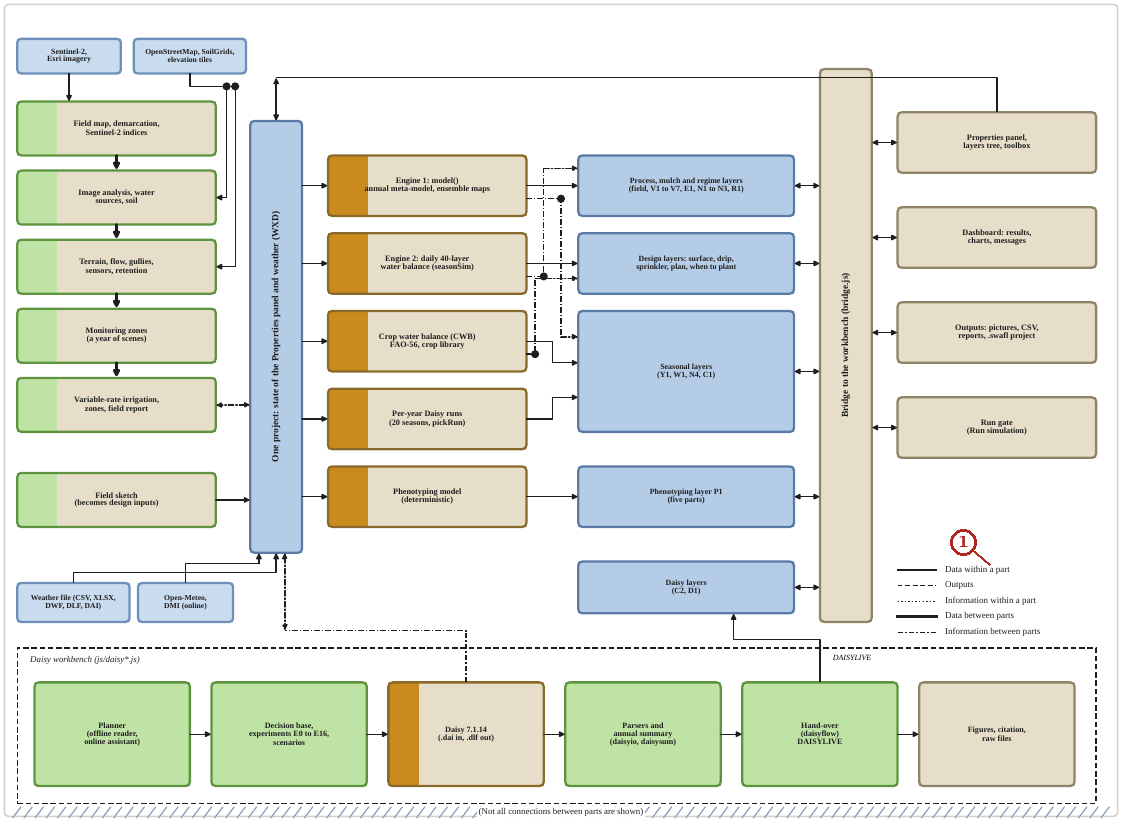
\includegraphics[width=\textwidth,height=0.42\textheight,keepaspectratio]{../figures/annot/p3_fig-system_0.png}\end{center}

\textbf{What the numbered labels point to.}
\begin{enumerate}[nosep,label=\protect\circled{\arabic*}]
\item Panel (a): see the caption above.
\end{enumerate}

\textbf{What it shows.} Architecture of SWAFL Desktop 1.1.0. The field tools (green) call the engines and write to the project; the project (blue bar) carries the state of the Properties panel and the weather to the five computing parts (brown); these feed the layers (blue); the layers and the workbench shell talk through one bridge; the Daisy workbench (dashed frame) hands its runs to the Daisy layers.

\textbf{How to read the labels, symbols and colours.} Architecture: green field tools, blue project and layers, brown computing parts, dashed frame the Daisy workbench; every arrow a dependency in the code.

\textbf{What affects it, and why it happens.} Everything passes through the project and one bridge, which is what makes the origin of every number traceable.

\textbf{How it is made.} Figure drawn by the script from the input data. Script: \nolinkurl{Manuscripts/reproducibility/p456/p456_figs_architecture.py}. Input: \nolinkurl{Data/daisy_ensemble.csv.gz}.


\subsection{Reading Figure 12 of the article}
\begin{center}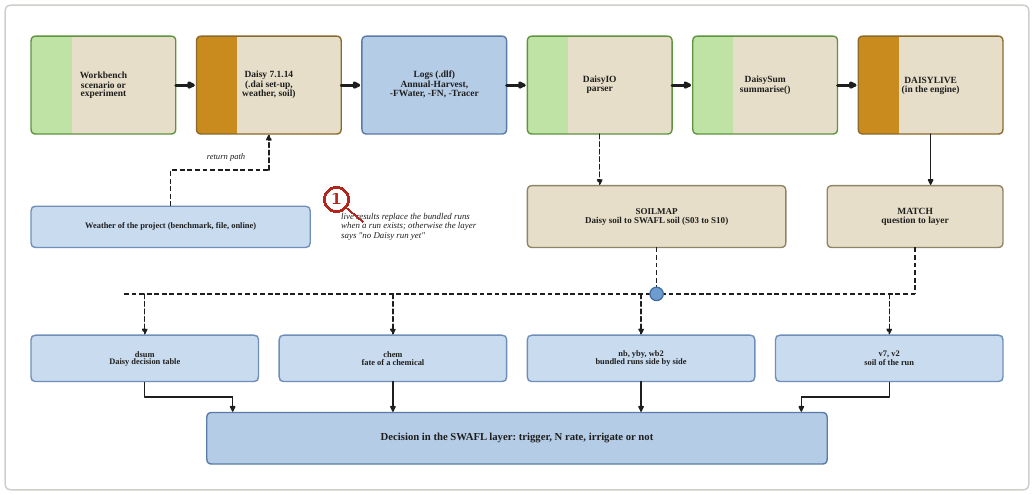
\includegraphics[width=\textwidth,height=0.42\textheight,keepaspectratio]{../figures/annot/p3_fig-bridge_0.png}\end{center}

\textbf{What the numbered labels point to.}
\begin{enumerate}[nosep,label=\protect\circled{\arabic*}]
\item Panel (a): see the caption above.
\end{enumerate}

\textbf{What it shows.} The bridge from a Daisy run to a decision. Heavy arrows are the path of a run, dashed arrows are outputs and the dashed arrow at the left is the return path of the weather of the project to Daisy.

\textbf{How to read the labels, symbols and colours.} Heavy arrows: path of a run; dashed: outputs; left dashed arrow: the project's weather back to Daisy.

\textbf{What affects it, and why it happens.} One bridge carries the values with their origin, which enforces the rule of origin.

\textbf{How it is made.} Figure drawn by the script from the input data. Script: \nolinkurl{Manuscripts/reproducibility/p456/p456_figs_schematics.py}. Input: \nolinkurl{Data/daisy_ensemble.csv.gz}.


\subsection{Reading Figure 17 of the article}
\begin{center}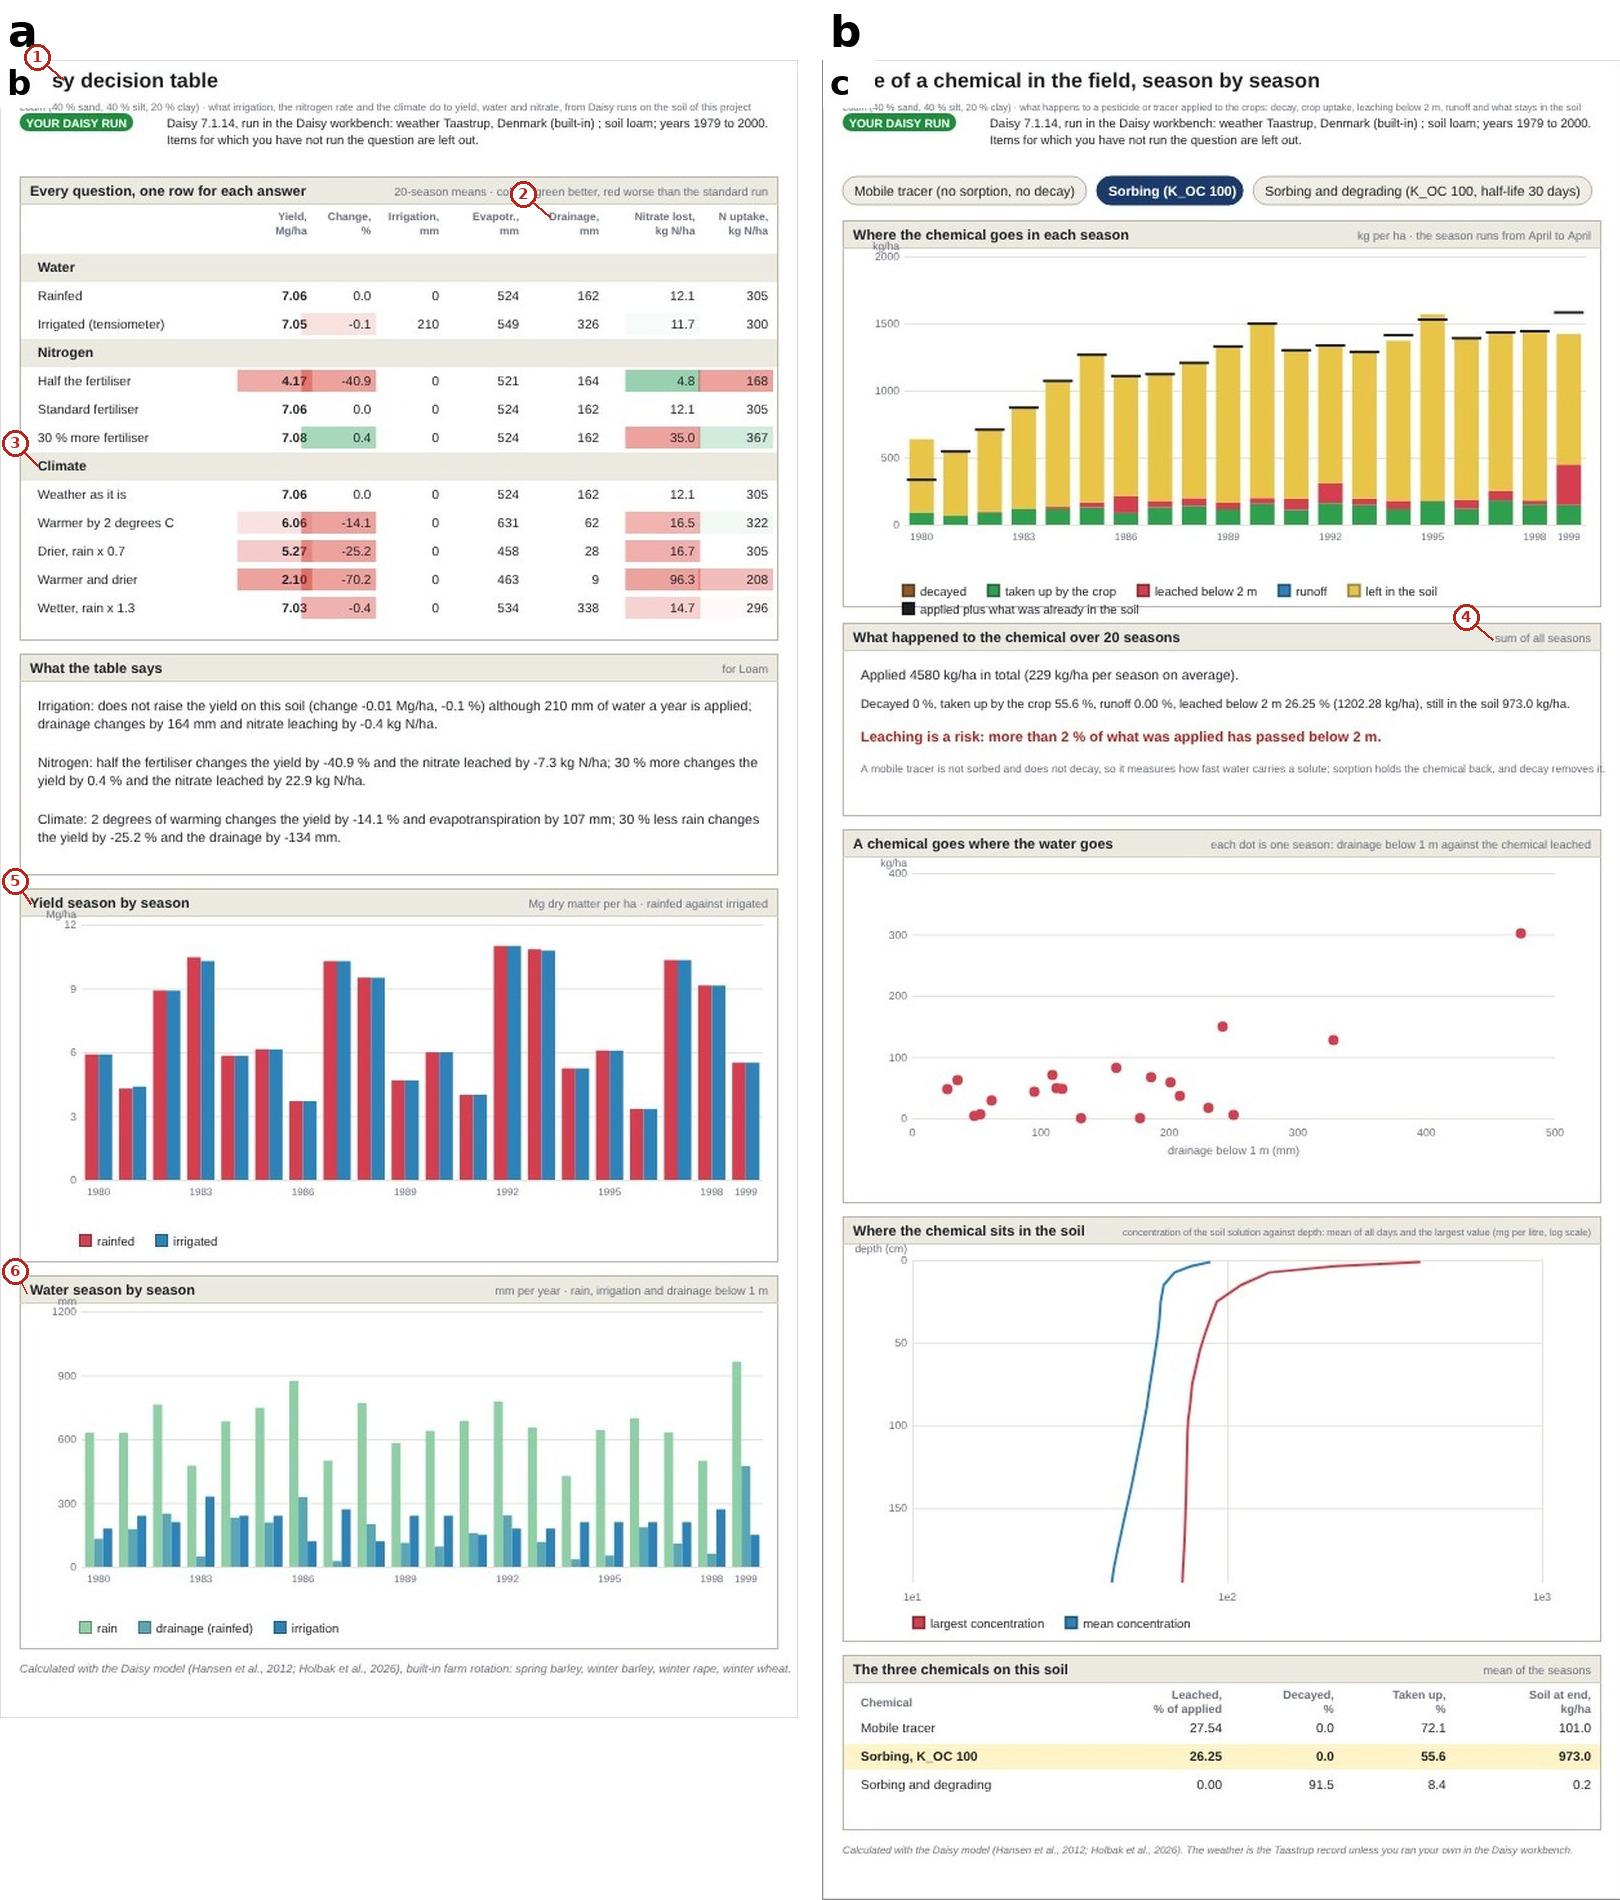
\includegraphics[width=\textwidth,height=0.42\textheight,keepaspectratio]{../figures/annot/p3_fig-flow_0.png}\end{center}

\textbf{What the numbered labels point to.}
\begin{enumerate}[nosep,label=\protect\circled{\arabic*}]
\item ``y decision table'': a heading or control of this screen; the caption above says which layer it belongs to.
\item ``Drainage'': rain, from the weather of the project.
\item ``Climate'': a heading or control of this screen; the caption above says which layer it belongs to.
\item ``sum of all seasons'': a heading or control of this screen; the caption above says which layer it belongs to.
\item ``Yield season by season'': a heading or control of this screen; the caption above says which layer it belongs to.
\item ``Water season by season'': a heading or control of this screen; the caption above says which layer it belongs to.
\end{enumerate}

\textbf{What it shows.} Results of the hand-over. (a) The Daisy decision table with the labels of the run (rainfed and irrigated, half and 30\,\% more fertiliser, warmer and drier climates). (b) The fate of a chemical for a mobile, a sorbing and a sorbing and degrading tracer.

\textbf{How to read the labels, symbols and colours.} (a) The decision table of the hand-over with run labels; (b) fate of three tracers.

\textbf{What affects it, and why it happens.} A mobile tracer leaches, a sorbing one stays, a sorbing and degrading one disappears in the soil.

\textbf{How it is made.} Screen capture of SWAFL Desktop 1.1.0 (not regenerated).


\subsection{Reading Figure 8 of the article}
\begin{center}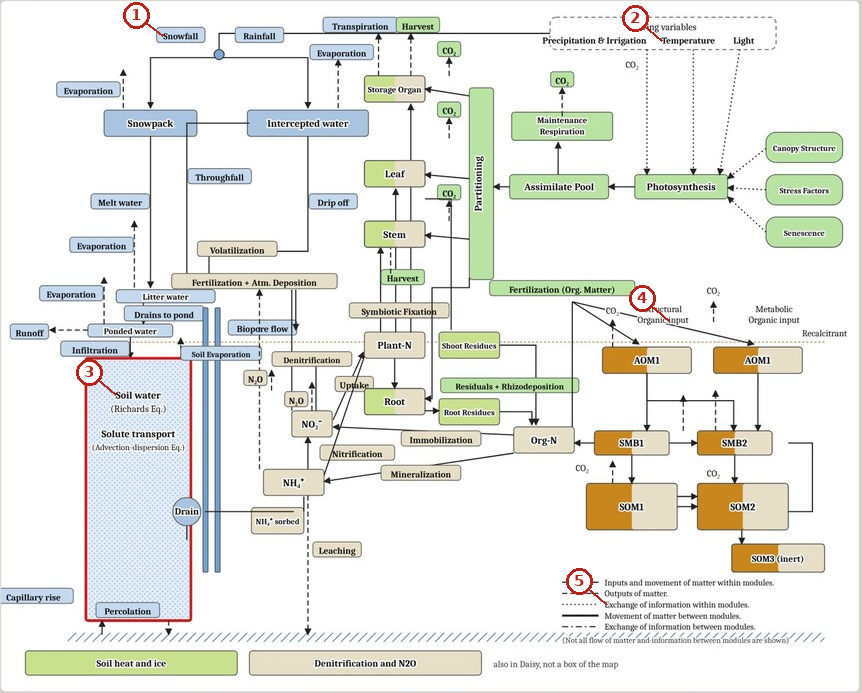
\includegraphics[width=\textwidth,height=0.42\textheight,keepaspectratio]{../figures/annot/p3_fig-screens_0.png}\end{center}

\textbf{What the numbered labels point to.}
\begin{enumerate}[nosep,label=\protect\circled{\arabic*}]
\item ``Snowfall'': a heading or control of this screen; the caption above says which layer it belongs to.
\item ``Temperature'': a heading or control of this screen; the caption above says which layer it belongs to.
\item ``Soil water'': the soil of the project, which every layer uses.
\item ``input'': a heading or control of this screen; the caption above says which layer it belongs to.
\item ``Exchange of information within modules'': a heading or control of this screen; the caption above says which layer it belongs to.
\end{enumerate}

\textbf{What it shows.} The process map of Daisy. Each process is a button that opens the figures it produces from a run.

\textbf{How to read the labels, symbols and colours.} The process map of Daisy; each box is a button.

\textbf{What affects it, and why it happens.} It shows which process produces which output, so a user finds the figure of a process.

\textbf{How it is made.} Screen capture of SWAFL Desktop 1.1.0 (not regenerated).


\subsection{Reading Figure 18 of the article}
\begin{center}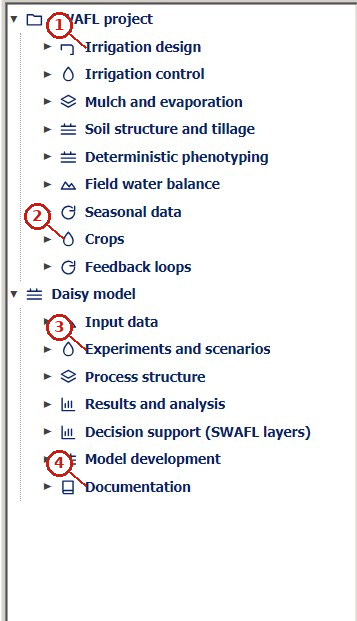
\includegraphics[width=\textwidth,height=0.42\textheight,keepaspectratio]{../figures/annot/p3_fig-ui11_0.png}\end{center}

\textbf{What the numbered labels point to (picture 1 of 3: The Layers panel: the nine groups of the SWAFL project and the seven of the Daisy model.).}
\begin{enumerate}[nosep,label=\protect\circled{\arabic*}]
\item ``Irrigation design'': the irrigation-design group of the Layers tree and its layers.
\item ``Crops'': the crop of the project and its stage.
\item ``Experiments and scenarios'': a heading or control of this screen; the caption above says which layer it belongs to.
\item ``Documentation'': a heading or control of this screen; the caption above says which layer it belongs to.
\end{enumerate}

\begin{center}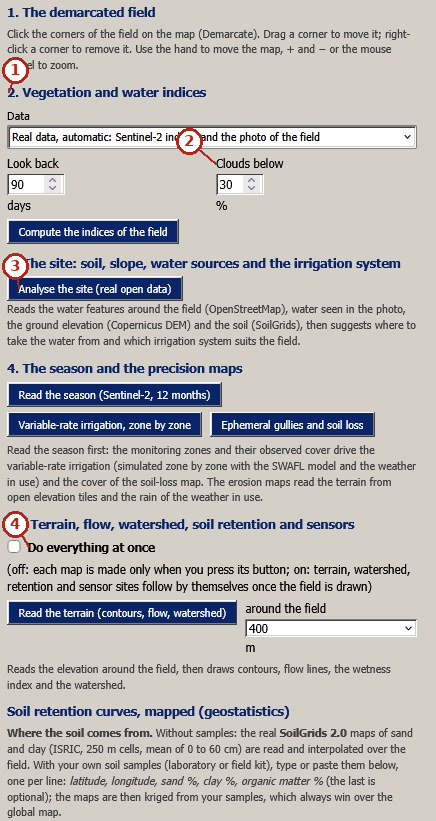
\includegraphics[width=\textwidth,height=0.42\textheight,keepaspectratio]{../figures/annot/p3_fig-ui11_1.png}\end{center}

\textbf{What the numbered labels point to (picture 2 of 3: The panel of the real field, sections 1 to 4b.).}
\begin{enumerate}[nosep,label=\protect\circled{\arabic*}]
\item ``2. Vegetation and water indices'': satellite indices of the vegetation computed from the Sentinel-2 bands.
\item ``Clouds below'': a heading or control of this screen; the caption above says which layer it belongs to.
\item ``Analyse the site (real open data)'': a heading or control of this screen; the caption above says which layer it belongs to.
\item ``Do everything at once'': a heading or control of this screen; the caption above says which layer it belongs to.
\end{enumerate}

\begin{center}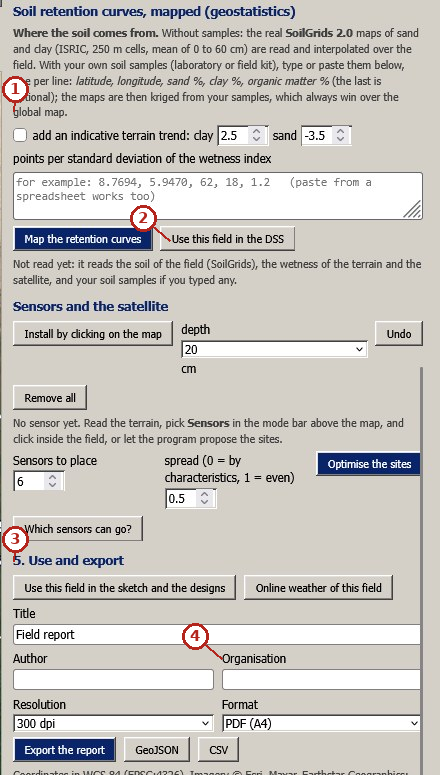
\includegraphics[width=\textwidth,height=0.42\textheight,keepaspectratio]{../figures/annot/p3_fig-ui11_2.png}\end{center}

\textbf{What the numbered labels point to (picture 3 of 3: Soil retention mapped, sensors, and export.).}
\begin{enumerate}[nosep,label=\protect\circled{\arabic*}]
\item ``global map'': a heading or control of this screen; the caption above says which layer it belongs to.
\item ``Use this field in the DSS'': a heading or control of this screen; the caption above says which layer it belongs to.
\item ``5. Use and export'': a heading or control of this screen; the caption above says which layer it belongs to.
\item ``Organisation'': a heading or control of this screen; the caption above says which layer it belongs to.
\end{enumerate}

\textbf{What it shows.} The interface of release 1.1.0 as it appears to the user (screen captures). Panels: (a) The Layers panel: the nine groups of the SWAFL project and the seven of the Daisy model. (b) The panel of the real field, sections 1 to 4b. (c) Soil retention mapped, sensors, and export.

\textbf{How to read the labels, symbols and colours.} Screens of the Layers panel and the field panel.

\textbf{What affects it, and why it happens.} The layers are grouped by question, so the user finds the layer that answers it. The groups organise the layers by question.

\textbf{How it is made.} Screen capture of SWAFL Desktop 1.1.0 (not regenerated).


\subsection{Why it happens}
\paragraph{Why every number can be traced.} Each value shown is computed by a function that carries the number of its equation and a label of origin (literature, fitted to data, engineered); the interface shows both, so the origin is a property of the code, not of the documentation.

\paragraph{Why a Daisy layer draws nothing before a Daisy run.} The rule of origin forbids a layer to show a Daisy result from any other source; without a run there is no result, so the layer says so rather than showing an example.

\paragraph{Why the routes from Daisy to a decision differ in time by orders of magnitude.} Running Daisy solves the Richards equation and a crop for every day of every run; the meta-model looks up and combines stored outcomes, which takes microseconds.


\section{Experiments within a run budget}
Designs that test every level of every factor within the budget the user sets.

\subsection{Contribution 2: an exact run budget that still tests every level}\label{con:s3:2}
\begin{problem}
A design of a few factors can need hundreds of Daisy runs of minutes each. How can the user set a budget and still test every level of every factor?
\end{problem}
\begin{derivation}
The full factorial is counted; if it exceeds the budget $B$, a Latin hypercube of $B$ runs is drawn in which the levels of each factor are used as evenly as possible.
\end{derivation}
\begin{keyresult}
\begin{pencil}
{\small\noindent\textbf{How it is derived, line by line}
\[\begin{array}{@{}l@{}}\textbf{1. Full factorial:}\\[1pt]
\qquad \textstyle\prod_in_i\\[1pt]
\textbf{2. Never above the budget:}\\[1pt]
\qquad N=\min(\prod_in_i,B)\\[1pt]
\textbf{3. Latin hypercube, levels balanced:}\\[1pt]
\qquad \text{each level used }\lfloor N/n_i\rfloor\text{ or }\lceil N/n_i\rceil\text{ times}
\end{array}\]}
\noindent\textbf{The result, with its parts marked}
\[\underbrace{N}_{\circled{1}}=\min\Bigl(\underbrace{\textstyle\prod_i n_i}_{\circled{2}},\ \underbrace{B}_{\circled{3}}\Bigr)\]
\[\underbrace{\text{each level of factor } i \text{ used } \lfloor N/n_i\rfloor \text{ or } \lceil N/n_i\rceil \text{ times}}_{\circled{4}}\]
\end{pencil}
\end{keyresult}
\begin{pins}
\pin{1}{The number of runs actually made, never above the budget.}
\pin{2}{The full factorial (for 4, 10 and 5 levels: 200 runs).}
\pin{3}{The budget set by the user (for example 60).}
\pin{4}{The Latin-hypercube choice spreads the runs so that every level appears almost equally often (each of the 10 levels 6 times), so main effects remain estimable.}
\end{pins}


\subsection{Worked numbers, part 6: keeping an experiment within its budget}
Three factors with 4, 10 and 5 levels make 200 combinations; with a budget of 60 runs a Latin-hypercube choice makes 60 runs in which each level of the second factor appears 6 times, so every level is still tested.


\subsection{Reading Figure 13 of the article}
\begin{center}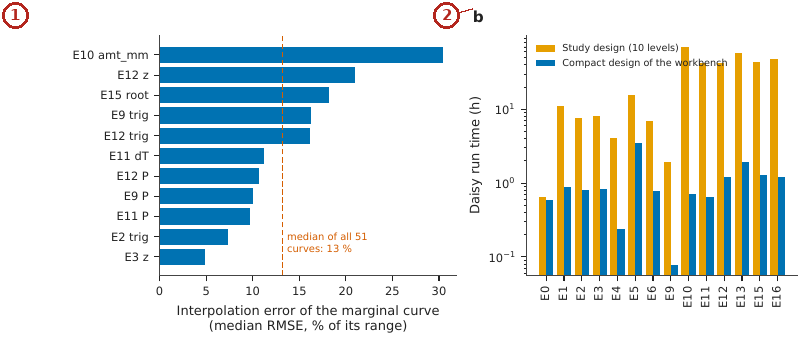
\includegraphics[width=\textwidth,height=0.42\textheight,keepaspectratio]{../figures/annot/p3_fig-fidelity_0.png}\end{center}

\textbf{What the numbered labels point to.}
\begin{enumerate}[nosep,label=\protect\circled{\arabic*}]
\item Panel (a): Error of the marginal curves rebuilt from the levels of the compact designs (median over five responses, per experiment and factor). \emph{Why:} Fewer levels miss the curvature between them, so curves rebuilt from compact designs err more where the response is curved.
\item Panel (b): Daisy run time of the study designs and of the compact designs, by experiment (logarithmic scale). \emph{Why:} Compact designs need orders of magnitude fewer runs, so far less Daisy time.
\end{enumerate}

\textbf{What it shows.} (a) Error of the marginal curves rebuilt from the levels of the compact designs (median over five responses, per experiment and factor). (b) Daisy run time of the study designs and of the compact designs, by experiment (logarithmic scale).

\textbf{How to read the labels, symbols and colours.} (a) Error of the marginal curves of the compact designs by experiment and factor; (b) Daisy time of the study and compact designs (log scale).

\textbf{What affects it, and why it happens.} Fewer levels miss curvature between them (error) but save orders of magnitude of time.

\textbf{How it is made.} Figure drawn by the script from the input data. Script: \nolinkurl{Manuscripts/reproducibility/p456/p456_figs_data.py}. Input: \nolinkurl{Data/daisy_ensemble.csv.gz}.


\subsection{Reading Figure 16 of the article}
\begin{center}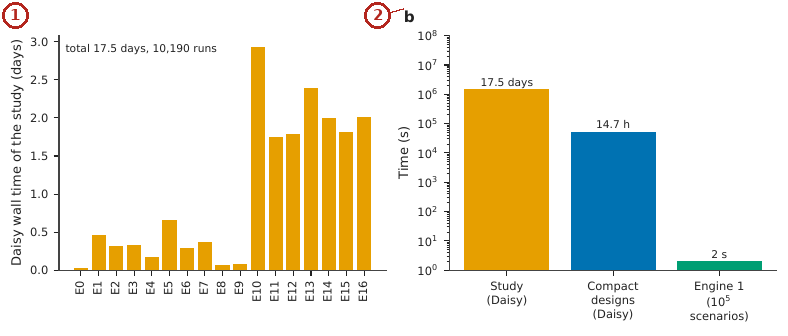
\includegraphics[width=\textwidth,height=0.42\textheight,keepaspectratio]{../figures/annot/p3_fig-econ_0.png}\end{center}

\textbf{What the numbered labels point to.}
\begin{enumerate}[nosep,label=\protect\circled{\arabic*}]
\item Panel (a): Daisy wall-clock time of the 17 experiments of the study (total 17.5 days). \emph{Why:} Experiments with more runs or longer runs take longer.
\item Panel (b): Time of the study, of the compact designs of the workbench and of Engine 1 for $10^5$ scenarios (logarithmic scale). \emph{Why:} Daisy solves every day of every run; the meta-model looks up stored results, so it is millions of times faster.
\end{enumerate}

\textbf{What it shows.} (a) Daisy wall-clock time of the 17 experiments of the study (total 17.5 days). (b) Time of the study, of the compact designs of the workbench and of Engine 1 for $10^5$ scenarios (logarithmic scale).

\textbf{How to read the labels, symbols and colours.} (a) Daisy time of each experiment; (b) time of the study, compact designs and Engine 1 (log scale).

\textbf{What affects it, and why it happens.} Each route trades fidelity for speed by orders of magnitude.

\textbf{How it is made.} Figure drawn by the script from the input data. Script: \nolinkurl{Manuscripts/reproducibility/p456/p456_figs_data.py}. Input: \nolinkurl{Data/daisy_ensemble.csv.gz}.


\subsection{Derivation: Run budget of an experiment}\label{der:s3:9}
For $k$ factors with $n_1,\dots,n_k$ levels the full design has $\prod n_i$ runs. When this exceeds the budget $B$ set by the user, a Latin-hypercube choice of $B$ runs is made: each factor's levels are used as evenly as possible ($B/n_i$ times each), so every level of every factor appears and the main effects remain estimable while the number of runs never exceeds $B$.


\subsection{Why it happens}
\paragraph{Why the compact designs lose some shape of a curve.} A design with fewer levels samples a curve at fewer points; the marginal curve is then drawn through those points and misses curvature between them, which is the loss measured.

\section{Root causes of failed runs}
The classes of Daisy failures and what to do about each.

\subsection{Contribution 3: the root cause of a failed run}\label{con:s3:3}
\begin{keyresult}
\centering\small
\begin{tabular}{lll}
\toprule
Daisy message contains & Class & What to do\\\midrule
\circled{1}\ Unknown '\dots' model & a name not defined & take only the needed definitions\\
\circled{2}\ did not converge, NaN & numerical & bring extreme values closer to typical\\
\circled{3}\ out of range, must be & range & change the level that writes the value\\
\circled{4}\ cannot open, not found & missing file & rerun; check the weather and soil\\\bottomrule
\end{tabular}
\end{keyresult}
\begin{pins}
\pin{1}{This class found a real defect: a file of the Daisy samples referred to logs of its own run; taking only the definitions a run needs removed it.}
\pin{2}{Numerical failures come from extreme hydraulic values; the message names the factor and the typical range.}
\pin{3}{The line and column of the set-up file are shown, so the user sees which input wrote the value.}
\pin{4}{Failed runs are grouped by cause, so one explanation covers all runs that failed for the same reason.}
\end{pins}


\subsection{Reading Figure 20 of the article}
\begin{center}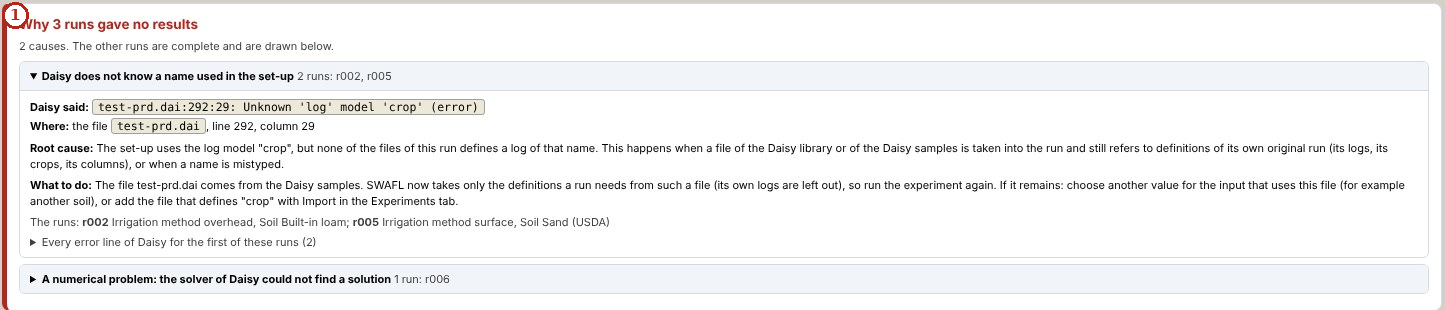
\includegraphics[width=\textwidth,height=0.42\textheight,keepaspectratio]{../figures/annot/p3_fig-diag_0.png}\end{center}

\textbf{What the numbered labels point to (picture 1 of 2: The root cause of runs that gave no results, grouped by cause, with the place in the set-up and what to do.).}
\begin{enumerate}[nosep,label=\protect\circled{\arabic*}]
\item ``Why 3 runs gave no results'': a heading or control of this screen; the caption above says which layer it belongs to.
\end{enumerate}

\begin{center}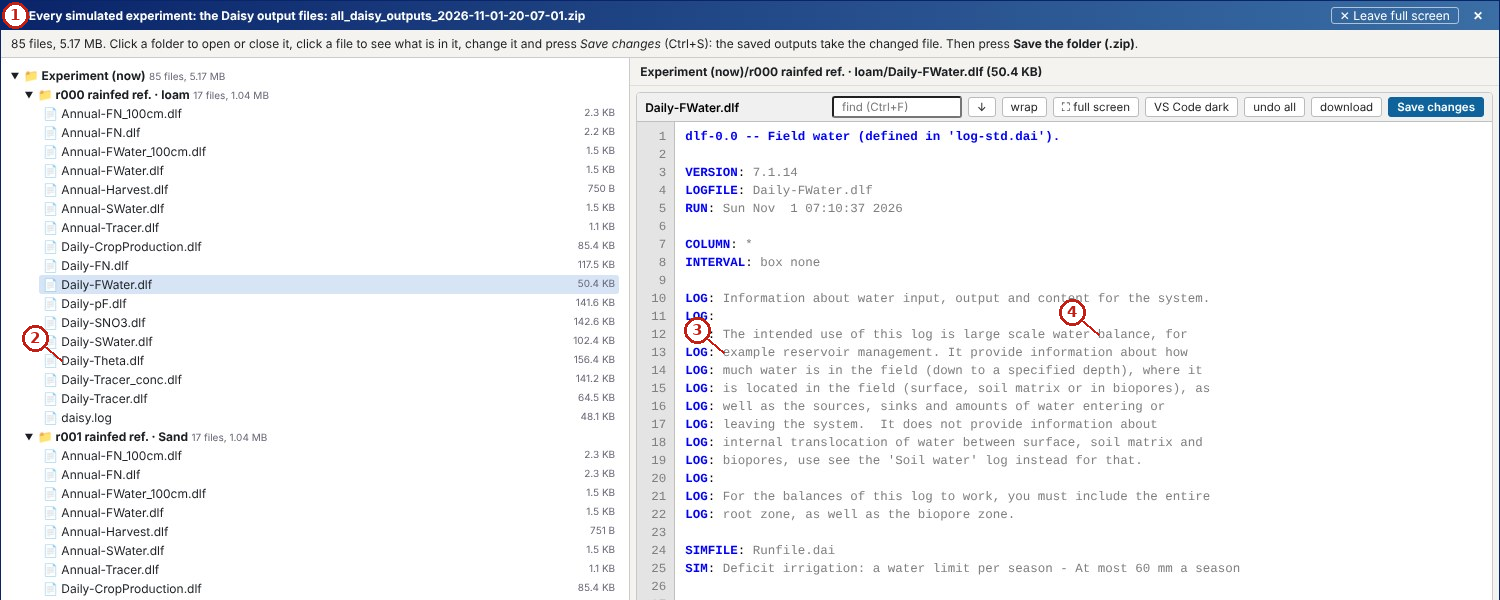
\includegraphics[width=\textwidth,height=0.42\textheight,keepaspectratio]{../figures/annot/p3_fig-diag_1.png}\end{center}

\textbf{What the numbered labels point to (picture 2 of 2: Every file Daisy wrote, experiment by experiment and run by run, in a full-screen viewer.).}
\begin{enumerate}[nosep,label=\protect\circled{\arabic*}]
\item ``Every simulated'': a heading or control of this screen; the caption above says which layer it belongs to.
\item ``Daily-Theta.dlf'': a heading or control of this screen; the caption above says which layer it belongs to.
\item ``example reservoir'': a heading or control of this screen; the caption above says which layer it belongs to.
\item ``balance'': a heading or control of this screen; the caption above says which layer it belongs to.
\end{enumerate}

\textbf{What it shows.} Diagnosis and provenance of the runs (screen captures). Panels: (a) The root cause of runs that gave no results, grouped by cause, with the place in the set-up and what to do. (b) Every file Daisy wrote, experiment by experiment and run by run, in a full-screen viewer.

\textbf{How to read the labels, symbols and colours.} Diagnosis of failed runs and the viewer of every file.

\textbf{What affects it, and why it happens.} Failed runs are grouped by the cause in Daisy's message, so one correction fixes every run that failed the same way. Errors are grouped by cause, so one fix addresses all runs that failed the same way.

\textbf{How it is made.} Screen capture of SWAFL Desktop 1.1.0 (not regenerated).


\subsection{Reading Figure 19 of the article}
\begin{center}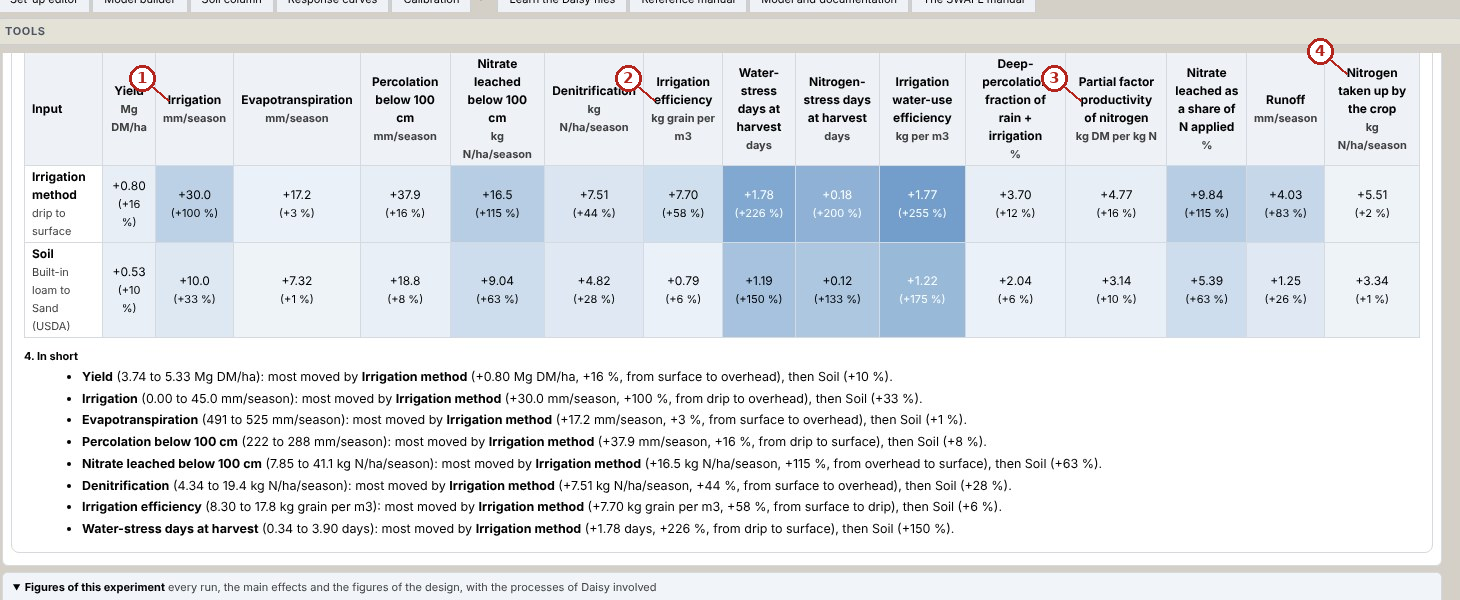
\includegraphics[width=\textwidth,height=0.42\textheight,keepaspectratio]{../figures/annot/p3_fig-engine_0.png}\end{center}

\textbf{What the numbered labels point to (picture 1 of 2: The summary of an experiment: the effect of every input on every result (blue rises, red falls; in brackets the share of the mean) and the summary in words.).}
\begin{enumerate}[nosep,label=\protect\circled{\arabic*}]
\item ``Irrigation'': a heading or control of this screen; the caption above says which layer it belongs to.
\item ``efficiency'': a heading or control of this screen; the caption above says which layer it belongs to.
\item ``productivity'': a heading or control of this screen; the caption above says which layer it belongs to.
\item ``Nitrogen'': a heading or control of this screen; the caption above says which layer it belongs to.
\end{enumerate}

\begin{center}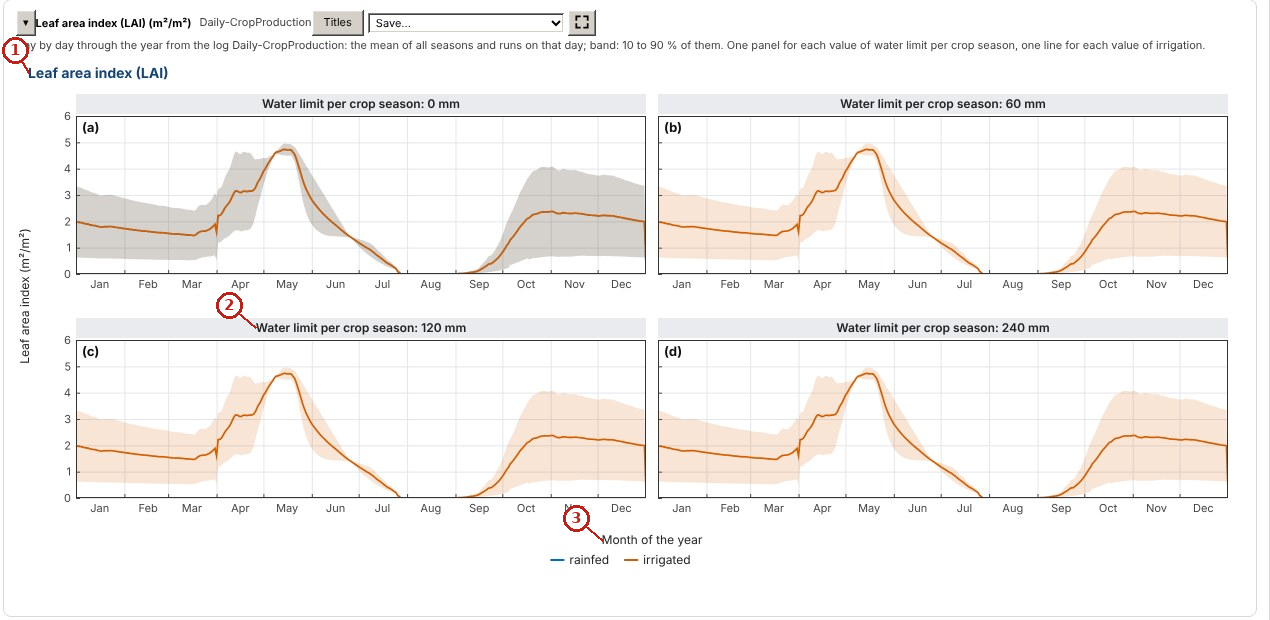
\includegraphics[width=\textwidth,height=0.42\textheight,keepaspectratio]{../figures/annot/p3_fig-engine_1.png}\end{center}

\textbf{What the numbered labels point to (picture 2 of 2: One of the figures of every log: leaf area index through the year, one panel per water limit, rainfed and irrigated, the mean of the seasons with 10 to 90\,\% as the band.).}
\begin{enumerate}[nosep,label=\protect\circled{\arabic*}]
\item ``Leaf area index (LAI)'': a heading or control of this screen; the caption above says which layer it belongs to.
\item ``Water limit per crop season: 120'': the crop of the project and its stage.
\item ``Month of the year'': a heading or control of this screen; the caption above says which layer it belongs to.
\end{enumerate}

\textbf{What it shows.} Outputs of the experiment engine drawn from Daisy runs (screen captures of the workbench). Panels: (a) The summary of an experiment: the effect of every input on every result (blue rises, red falls; in brackets the share of the mean) and the summary in words. (b) One of the figures of every log: leaf area index through the year, one panel per water limit, rainfed and irrigated, the mean of the seasons with 10 to 90\,\% as the band.

\textbf{How to read the labels, symbols and colours.} Summary of an experiment (blue rises, red falls) and a figure of one log.

\textbf{What affects it, and why it happens.} The effect of each input is the change of each result across its levels, so the largest bars are the inputs that matter most. Each input's effect on each result is its range across the runs, shown with sign.

\textbf{How it is made.} Screen capture of SWAFL Desktop 1.1.0 (not regenerated).


\subsection{Why it happens}
\paragraph{Why runs on a horizon of the Daisy samples failed.} The sample file also defined logs that referred to a model of its original run; Daisy stopped on the unknown name. Taking only the definitions a run needs removed the error.

\section{The soil column and its hydraulic factors}
The Richards equation of the column and the factors that rewrite every horizon.

\subsection{Contribution 4: soil-hydraulic factors for every horizon}\label{con:s3:4}
\begin{derivation}
Each factor rewrites the hydraulic block of every horizon of the set-up file before Daisy runs; $n-1$ rather than $n$ is scaled so that $n>1$ for any factor; one run of the loam was made with Daisy 7.1.14 with and without the factors.
\end{derivation}
\begin{keyresult}
\begin{pencil}
{\small\noindent\textbf{How it is derived, line by line}
\[\begin{array}{@{}l@{}}\textbf{1. Keep } n>1\textbf{ for any factor by scaling } n-1\textbf{:}\\[1pt]
\qquad n'=1+f_n(n-1)\\[1pt]
\textbf{2. Scale the other parameters of every horizon:}\\[1pt]
\qquad K_s'=f_kK_s,\ \alpha'=f_a\alpha,\ \theta_s'=f_t\theta_s,\ \ell'=\ell+\delta\ell
\end{array}\]}
\noindent\textbf{The result, with its parts marked}
\[\underbrace{K_s\to f_kK_s}_{\circled{1}},\quad \underbrace{\alpha\to f_a\alpha}_{\circled{2}},\quad \underbrace{n-1\to f_n(n-1)}_{\circled{3}},\quad \theta_s\to f_t\theta_s,\quad \ell\to\ell+\delta\ell\]
\[\underbrace{\text{percolation }177\to222\ \mathrm{mm}}_{\circled{4}}\]
\end{pencil}
\end{keyresult}
\begin{pins}
\pin{1}{Scaling the saturated conductivity of every horizon at once keeps the layering of the soil.}
\pin{2}{Scaling $\alpha$ moves the air-entry suction.}
\pin{3}{Scaling $n-1$ (not $n$) keeps $n>1$, so the van~Genuchten curve stays valid for any factor.}
\pin{4}{A faster-draining parameter set, run end to end with Daisy, raised one season's matrix percolation from 177 to 222\,mm and removed runoff, the direction expected from the conductivity.}
\end{pins}


\subsection{Reading Figure 14 of the article}
\begin{center}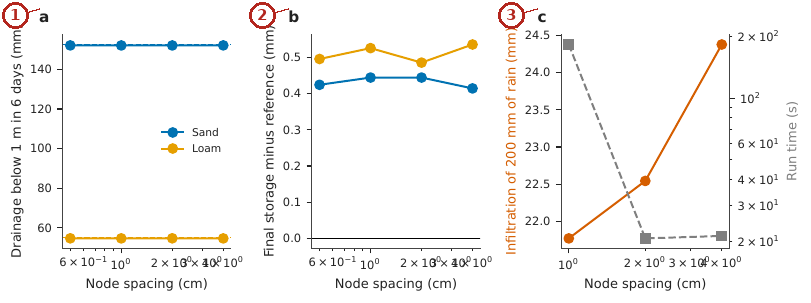
\includegraphics[width=\textwidth,height=0.42\textheight,keepaspectratio]{../figures/annot/p3_fig-richards_0.png}\end{center}

\textbf{What the numbered labels point to.}
\begin{enumerate}[nosep,label=\protect\circled{\arabic*}]
\item Panel (a): Drainage below 1\,m with the node spacing; dashed lines are the reference. \emph{Why:} Coarser node spacing smooths wetting fronts, so drainage departs from the fine-grid reference.
\item Panel (b): Final storage minus the reference. \emph{Why:} Storage errors follow the drainage errors because water must be conserved.
\item Panel (c): Infiltration of 200\,mm of rain into a ponded silty clay loam (left axis) and run time (right axis), showing the lack of convergence. \emph{Why:} A ponded fine soil has very steep suction gradients at the surface and tiny conductivity, so the solver needs tiny steps and does not converge in reasonable time.
\end{enumerate}

\textbf{What it shows.} Soil column. (a) Drainage below 1\,m with the node spacing; dashed lines are the reference. (b) Final storage minus the reference. (c) Infiltration of 200\,mm of rain into a ponded silty clay loam (left axis) and run time (right axis), showing the lack of convergence.

\textbf{How to read the labels, symbols and colours.} (a) Drainage below 1\,m against node spacing, dashed reference; (b) storage error; (c) infiltration into a ponded fine soil and run time.

\textbf{What affects it, and why it happens.} Coarser grids smooth the fronts; a ponded fine soil has steep gradients and tiny conductivity, so the solver needs small steps and does not converge in reasonable time.

\textbf{How it is made.} Figure drawn by the script from the input data. Script: \nolinkurl{Manuscripts/reproducibility/p456/p456_figs_data.py}. Input: \nolinkurl{Data/daisy_ensemble.csv.gz}.


\subsection{Reading Figure 9 of the article}
\begin{center}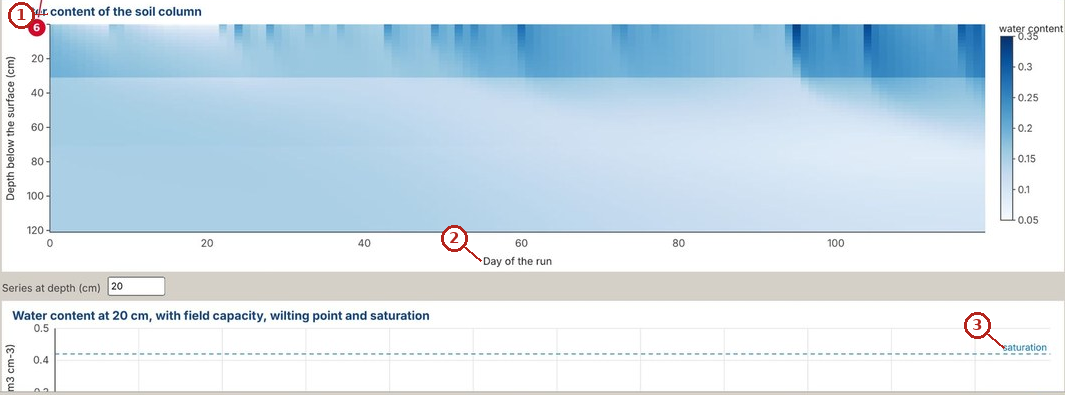
\includegraphics[width=\textwidth,height=0.42\textheight,keepaspectratio]{../figures/annot/p3_fig-column_0.png}\end{center}

\textbf{What the numbered labels point to.}
\begin{enumerate}[nosep,label=\protect\circled{\arabic*}]
\item ``content of the soil column'': the soil of the project, which every layer uses.
\item ``Day of the run'': a heading or control of this screen; the caption above says which layer it belongs to.
\item ``saturation'': a heading or control of this screen; the caption above says which layer it belongs to.
\end{enumerate}

\textbf{What it shows.} Water content of a soil column through time, computed by the Richards solver of the workbench.

\textbf{How to read the labels, symbols and colours.} Water content through depth and time from the column solver; colour is water content.

\textbf{What affects it, and why it happens.} Wetting fronts move down after rain and the profile dries from the top by evaporation and uptake.

\textbf{How it is made.} Screen capture of SWAFL Desktop 1.1.0 (not regenerated).


\subsection{Derivation: The Richards equation of the soil column}\label{der:s3:4}
Mass conservation of water in a layer of thickness $\dd z$ gives $\partial\theta/\partial t=-\partial q/\partial z-S$, with $S$ the root uptake. The Darcy--Buckingham flux with $z$ positive downward and $h$ the suction head is $q=K(h)(1-\partial h/\partial z)$: gravity drives water down and a suction gradient drives it towards the drier soil. With $\theta(h)$ and $K(h)$ from the van~Genuchten--Mualem functions the equation is closed and is solved implicitly with Picard iteration in the column of the workbench.


\subsection{Why it happens}
\paragraph{Why the soil column is slow for a ponded fine soil.} With ponding the top boundary is a fixed head and the fine soil has a very small conductivity and a steep head gradient at the surface; the implicit solver then needs small time steps and many iterations to converge.

\section{Nitrogen and the denitrification split}
The nitrogen budget and the defect found in a shared function.

\subsection{Contribution 5: a defect found in a shared function}\label{con:s3:5}
\begin{problem}
The denitrification function is shared with Daisy's Python tools. Is the copy used by the software right?
\end{problem}
\begin{derivation}
The function was evaluated on the stored inputs of the 792 cases distributed with Daisy's tools and its outputs compared case by case with Daisy's stored results.
\end{derivation}
\begin{keyresult}
\begin{pencil}
{\small\noindent\textbf{How it is derived, line by line}
\[\begin{array}{@{}l@{}}\textbf{1. Run the function on the stored inputs:}\\[1pt]
\qquad D_j^{\text{SWAFL}},\ j=1..792\\[1pt]
\textbf{2. Compare case by case:}\\[1pt]
\qquad \max_j|D_j^{\text{SWAFL}}-D_j^{\text{Daisy}}|
\end{array}\]}
\noindent\textbf{The result, with its parts marked}
\[\underbrace{\max_{j=1..792}\bigl|D_j^{\text{SWAFL}}-D_j^{\text{Daisy}}\bigr|}_{\circled{1}}\quad\Rightarrow\quad\underbrace{\text{one branch wrong, corrected}}_{\circled{2}}\]
\end{pencil}
\end{keyresult}
\begin{pins}
\pin{1}{The function was evaluated on the 792 cases for which Daisy's own results are stored, and compared case by case.}
\pin{2}{One class of cases disagreed; the branch responsible was found and corrected, after which the cases agree. A shared function was tested rather than trusted.}
\end{pins}

\subsection{Worked numbers, part 7: splitting denitrification}
With 12\,kg\,N\,ha$^{-1}$ denitrified and an N$_2$:N$_2$O ratio of 4, N$_2$O $=12/5=2.4$ and N$_2=9.6$\,kg\,N\,ha$^{-1}$.


\subsection{Reading Figure 15 of the article}
\begin{center}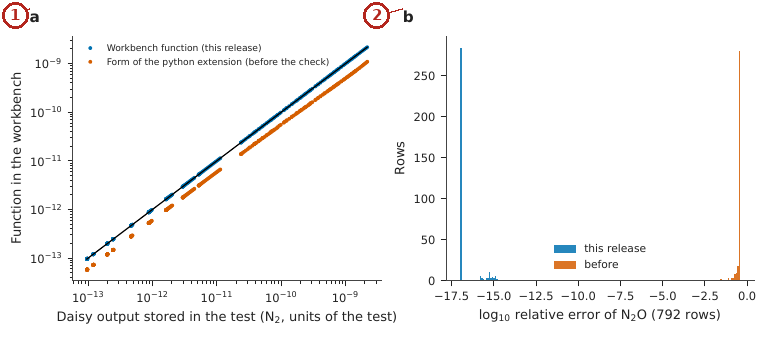
\includegraphics[width=\textwidth,height=0.42\textheight,keepaspectratio]{../figures/annot/p3_fig-deni_0.png}\end{center}

\textbf{What the numbered labels point to.}
\begin{enumerate}[nosep,label=\protect\circled{\arabic*}]
\item Panel (a): N$_2$ loss; the 1:1 line is black. \emph{Why:} After the correction the function and Daisy agree, so points lie on the 1:1 line.
\item Panel (b): Histogram of the relative error of the N$_2$O loss before and after the correction. \emph{Why:} Before the correction one class of cases had large errors; after it the errors collapse to zero.
\end{enumerate}

\textbf{What it shows.} Denitrification function against the 792 stored Daisy outputs. (a) N$_2$ loss; the 1:1 line is black. (b) Histogram of the relative error of the N$_2$O loss before and after the correction.

\textbf{How to read the labels, symbols and colours.} (a) N$_2$ loss of the function against 792 stored Daisy outputs, 1:1 line; (b) histogram of the N$_2$O error before and after the correction.

\textbf{What affects it, and why it happens.} Before the correction one class of cases was off; after it, the errors collapse to zero.

\textbf{How it is made.} Figure drawn by the script from the input data. Script: \nolinkurl{Manuscripts/reproducibility/p456/p456_figs_data.py}. Input: \nolinkurl{Data/daisy_ensemble.csv.gz}.


\subsection{Derivation: Nitrogen and chemical budgets}\label{der:s3:5}
For each season, the change of the mineral nitrogen store equals inputs minus outputs: fertiliser, deposition and mineralisation in; uptake, leaching, denitrification and volatilisation out. For a chemical, $\Delta M=A-U-L-R-X$ (applied, taken up, leached by every route, run off, transformed); the bridge reads each term from the Daisy logs and the closure of this budget is its test.


\subsection{Derivation: Splitting denitrification into N$_2$O and N$_2$}\label{der:s3:6}
Let $r$ be the ratio of N$_2$ to N$_2$O in the gaseous product of denitrification $D$. Then $D_{\mathrm{N_2O}}+D_{\mathrm{N_2}}=D$ and $D_{\mathrm{N_2}}=r\,D_{\mathrm{N_2O}}$, so $D_{\mathrm{N_2O}}(1+r)=D$, giving $D_{\mathrm{N_2O}}=D/(1+r)$ and $D_{\mathrm{N_2}}=rD/(1+r)=D/(1+1/r)$, the two expressions of the paper. The ratio is the smaller of a nitrate and a carbon-dioxide limited ratio, scaled by a water factor, so wetter, more active soils give relatively more N$_2$.


\subsection{Why it happens}
\paragraph{Why the denitrification defect was found.} The check compared the shared function with the stored Daisy results over 792 cases; one case class disagreed, which pointed to a wrong branch in the function, corrected in the release.

\section{Maps of the field}
Vegetation indices, crop coefficient, water balance, terrain, wetness and soil loss of every map cell.

\subsection{Worked numbers, part 1: a vegetation index from a satellite pixel}
Green leaves reflect near-infrared light and absorb red light. \emph{Example:} near-infrared reflectance 0.28 and red 0.11 give $\mathrm{NDVI}=(0.28-0.11)/(0.28+0.11)=0.44$, a moderately green crop.


\subsection{Worked numbers, part 2: the crop coefficient of the day}
FAO-56 describes the crop's water use relative to a reference grass with four straight lines. \emph{Example:} with stages of 30, 40, 50 and 30 days and $K_c$ of 0.40, 1.15 and 0.40, day 50 lies in the development stage: $K_c=0.40+(1.15-0.40)\times(50-30)/40=0.78$; day 70 starts the mid-season, $K_c=1.15$.


\subsection{Worked numbers, part 3: the daily water balance of a map cell}
Each 10\,m cell keeps a root-zone depletion: yesterday's depletion minus rain and irrigation plus crop water use; when it passes the readily available water, the cell needs irrigation of that depth.


\subsection{Worked numbers, part 4: soil loss}
$A=R\,K\,LS\,C\,P$. \emph{Example:} $450\times0.03\times0.4\times0.3\times1=1.6$\,t\,ha$^{-1}$\,yr$^{-1}$, below a tolerable 2\,t.


\subsection{Worked numbers, part 5: where the soil stays wet}
The wetness index is $\ln(a/\tan\beta)$. \emph{Example:} 250\,m of upslope area per metre of contour on a slope of 1.9$^\circ$ gives $\ln(250/0.0332)=8.9$, a wet position.


\subsection{Reading Figure 2 of the article}
\begin{center}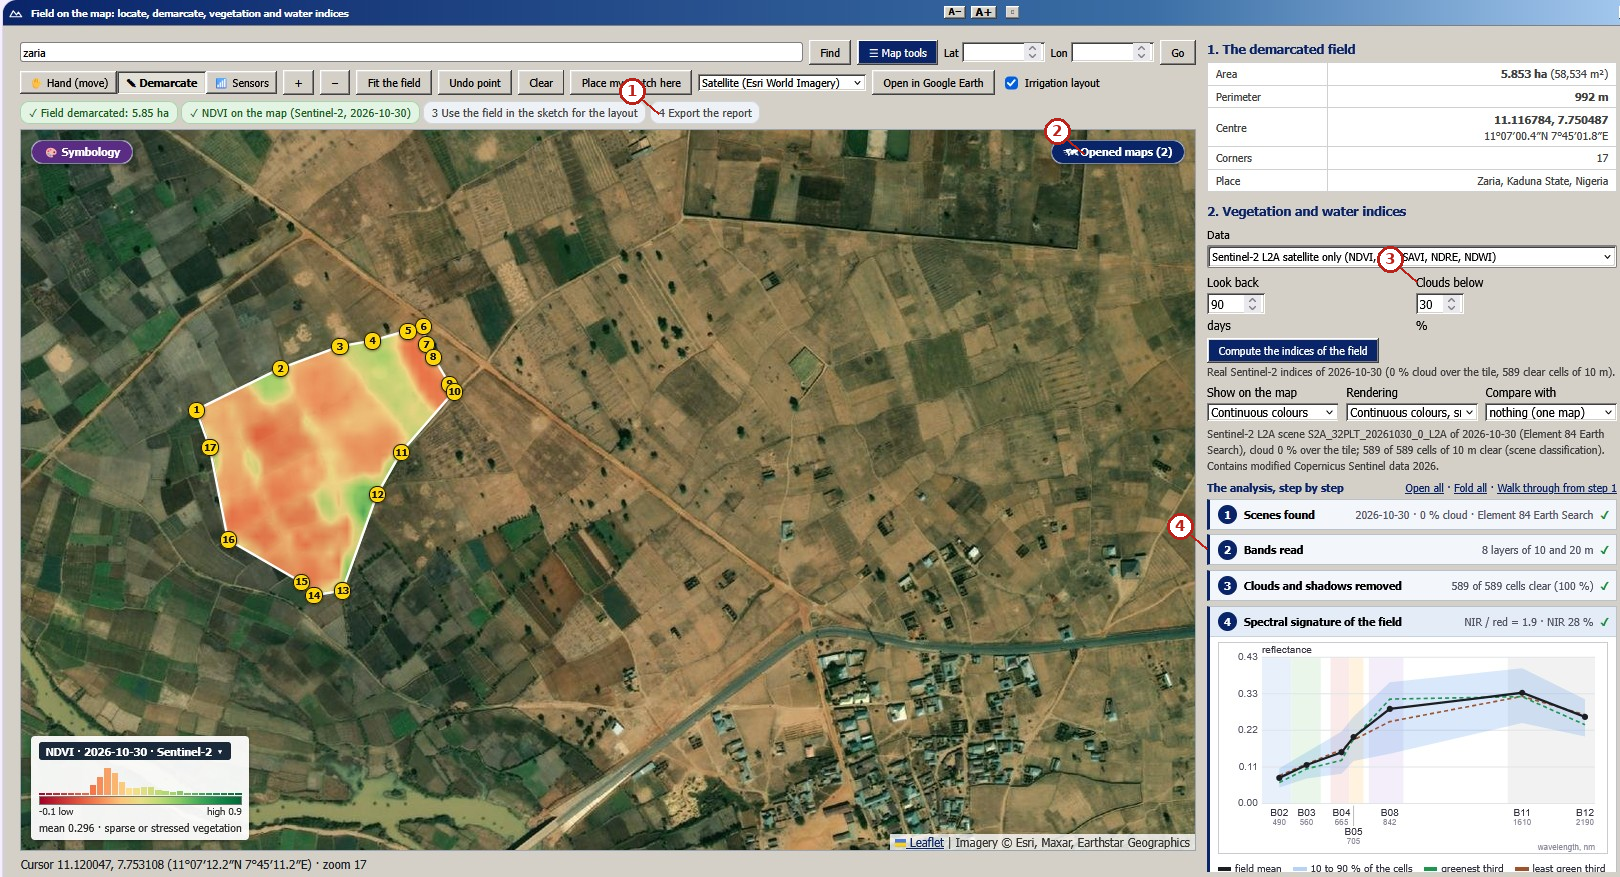
\includegraphics[width=\textwidth,height=0.42\textheight,keepaspectratio]{../figures/annot/p3_fig-zaria1_0.png}\end{center}

\textbf{What the numbered labels point to (picture 1 of 3: The demarcated field (5.85~ha) with the NDVI of the Sentinel-2 scene of 30 October 2026 cut to its outline, the legend with the histogram of the field, and the analysis step by step with the spectral signature of the field.).}
\begin{enumerate}[nosep,label=\protect\circled{\arabic*}]
\item ``Export the report'': export of the field report and its maps.
\item ``Opened maps (2)'': a heading or control of this screen; the caption above says which layer it belongs to.
\item ``Clouds below'': a heading or control of this screen; the caption above says which layer it belongs to.
\item ``Bands read'': satellite indices of the vegetation computed from the Sentinel-2 bands.
\end{enumerate}

\begin{center}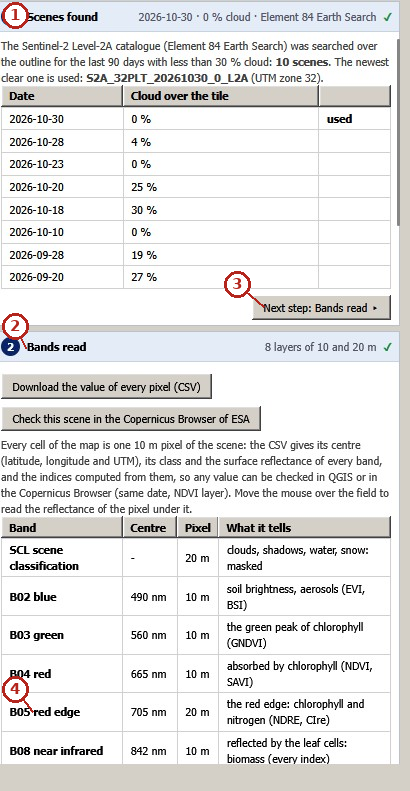
\includegraphics[width=\textwidth,height=0.42\textheight,keepaspectratio]{../figures/annot/p3_fig-zaria1_1.png}\end{center}

\textbf{What the numbered labels point to (picture 2 of 3: The scenes found and the bands read.).}
\begin{enumerate}[nosep,label=\protect\circled{\arabic*}]
\item ``Scenes found'': a heading or control of this screen; the caption above says which layer it belongs to.
\item ``Bands read'': satellite indices of the vegetation computed from the Sentinel-2 bands.
\item ``Next step'': moves to the next or previous step of the guided path.
\item ``red edge'': a heading or control of this screen; the caption above says which layer it belongs to.
\end{enumerate}

\begin{center}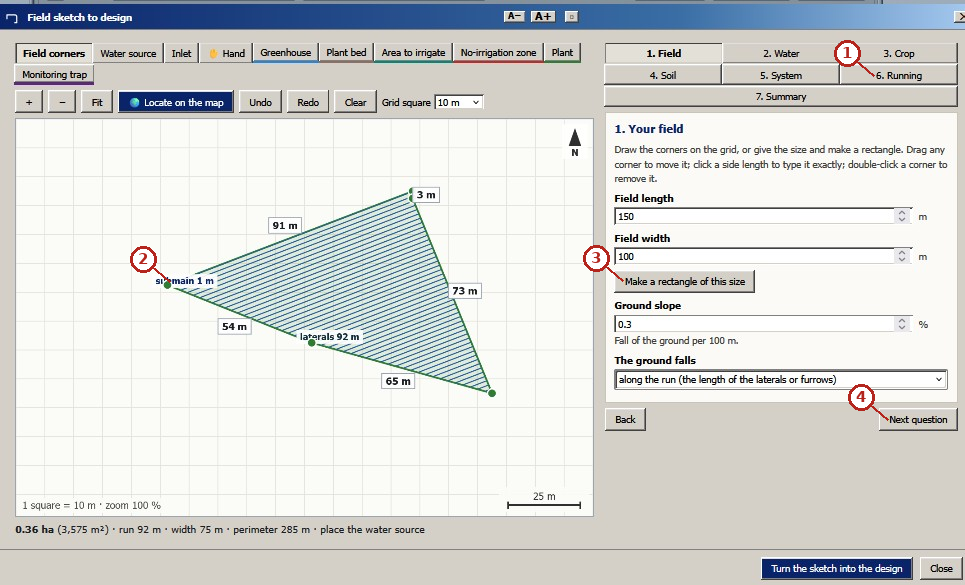
\includegraphics[width=\textwidth,height=0.42\textheight,keepaspectratio]{../figures/annot/p3_fig-zaria1_2.png}\end{center}

\textbf{What the numbered labels point to (picture 3 of 3: The field sketch that carries a field into the designs.).}
\begin{enumerate}[nosep,label=\protect\circled{\arabic*}]
\item ``6. Running'': a heading or control of this screen; the caption above says which layer it belongs to.
\item ``main 1m'': a heading or control of this screen; the caption above says which layer it belongs to.
\item ``Make a rectangle of this size'': a heading or control of this screen; the caption above says which layer it belongs to.
\item ``Next question'': moves to the next or previous step of the guided path.
\end{enumerate}

\textbf{What it shows.} A real field near Zaria, Nigeria: demarcation and satellite indices (screen captures of release 1.1.0). Panels: (a) The demarcated field (5.85~ha) with the NDVI of the Sentinel-2 scene of 30 October 2026 cut to its outline, the legend with the histogram of the field, and the analysis step by step with the spectral signature of the field. (b) The scenes found and the bands read. (c) The field sketch that carries a field into the designs.

\textbf{How to read the labels, symbols and colours.} Screens of the real field: NDVI map with its histogram and spectral signature, the scenes and bands, and the sketch of the field.

\textbf{What affects it, and why it happens.} Greener cells reflect more near-infrared and less red light, so NDVI is higher where the crop is denser. Greener cells (higher NDVI) have more active vegetation; the scene is the clearest of the last 90 days.

\textbf{How it is made.} Screen capture of SWAFL Desktop 1.1.0 (not regenerated).


\subsection{Reading Figure 3 of the article}
\begin{center}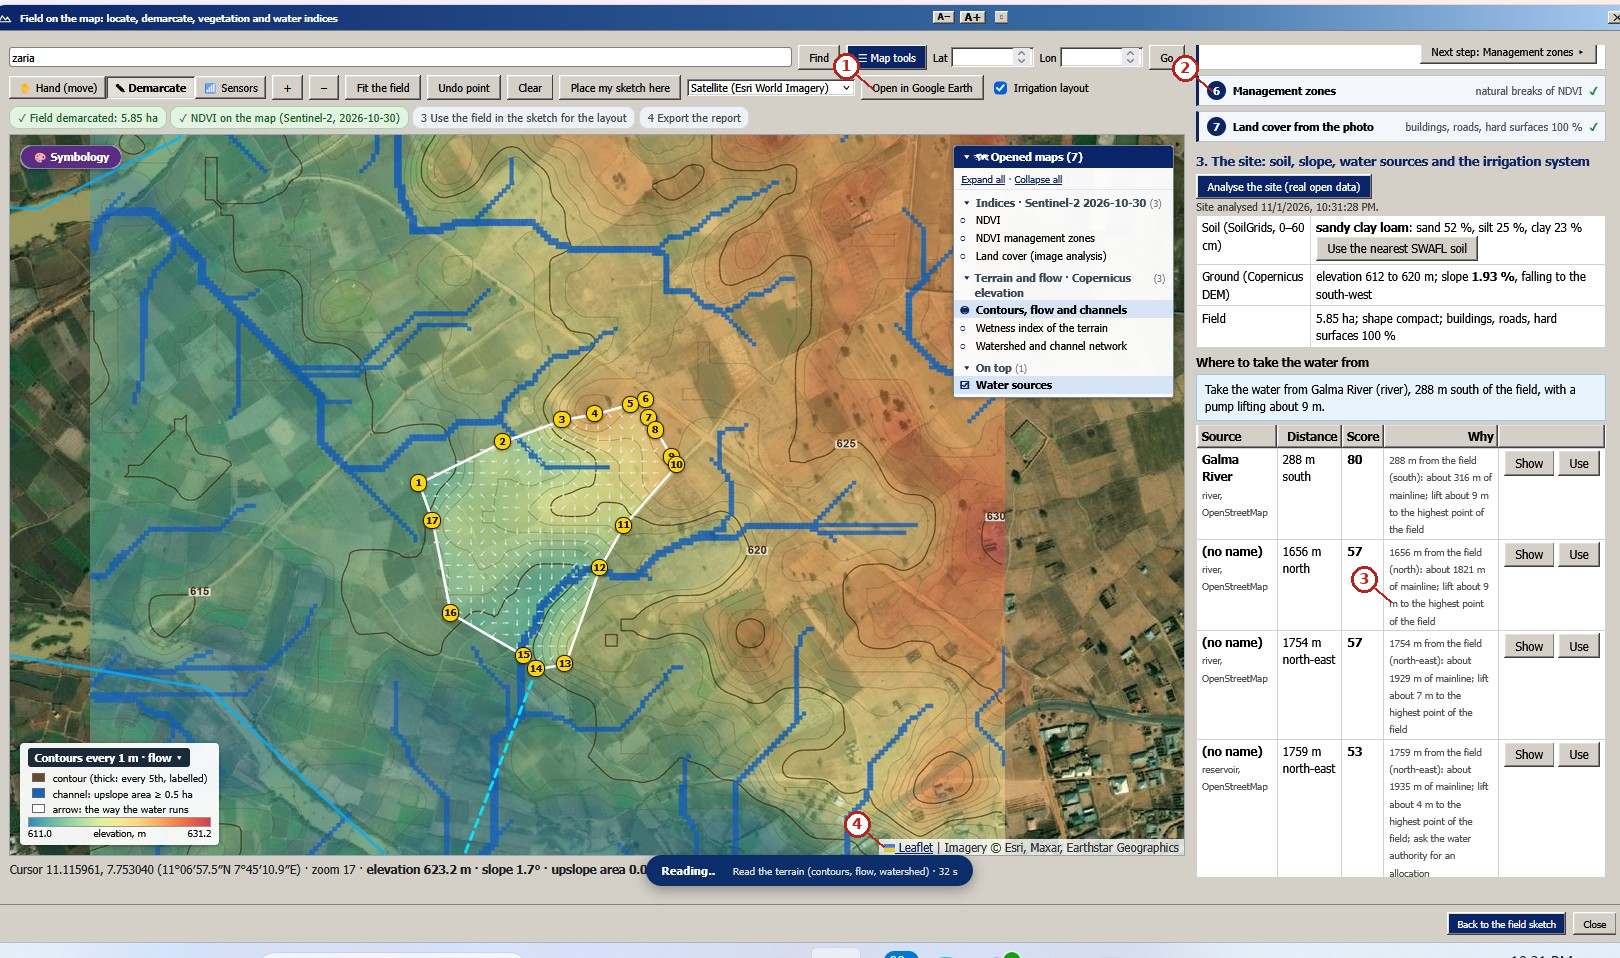
\includegraphics[width=\textwidth,height=0.42\textheight,keepaspectratio]{../figures/annot/p3_fig-zaria2_0.png}\end{center}

\textbf{What the numbered labels point to (picture 1 of 4: Contours every metre, flow arrows and channels, and the ranked water sources.).}
\begin{enumerate}[nosep,label=\protect\circled{\arabic*}]
\item ``Open in Google Earth'': a heading or control of this screen; the caption above says which layer it belongs to.
\item ``zones'': a heading or control of this screen; the caption above says which layer it belongs to.
\item ``m to the highest point'': a heading or control of this screen; the caption above says which layer it belongs to.
\item ``Imagery ©'': a heading or control of this screen; the caption above says which layer it belongs to.
\end{enumerate}

\begin{center}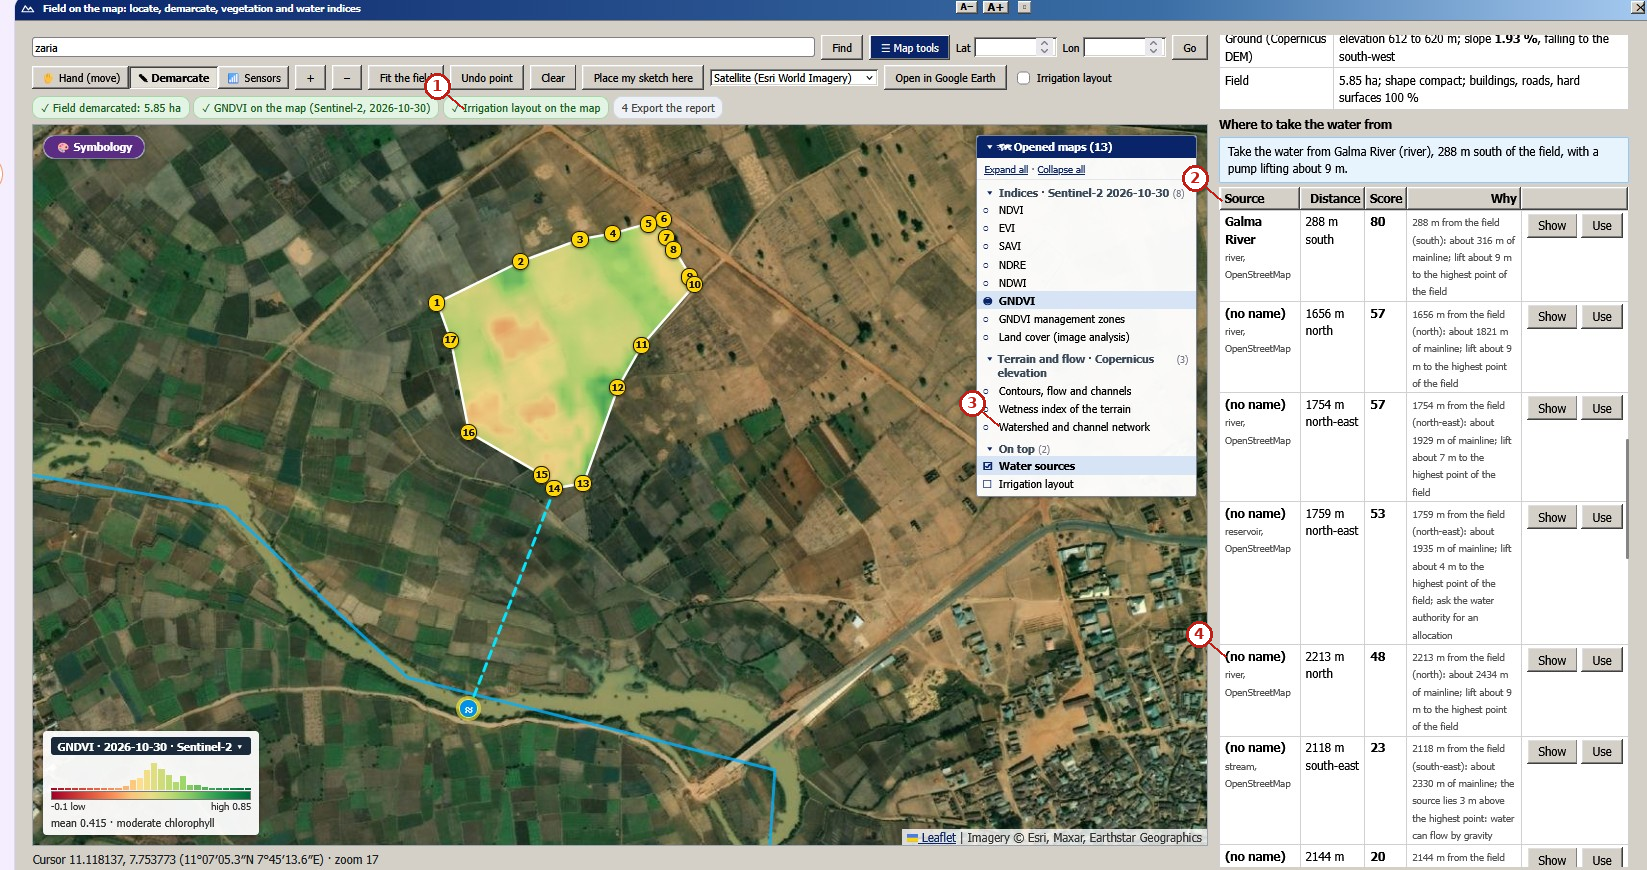
\includegraphics[width=\textwidth,height=0.42\textheight,keepaspectratio]{../figures/annot/p3_fig-zaria2_1.png}\end{center}

\textbf{What the numbered labels point to (picture 2 of 4: GNDVI and the line to the best water source, the Galma River (288~m).).}
\begin{enumerate}[nosep,label=\protect\circled{\arabic*}]
\item ``Irrigation layout on the map'': a heading or control of this screen; the caption above says which layer it belongs to.
\item ``Source Score'': a heading or control of this screen; the caption above says which layer it belongs to.
\item ``Watershed and channel network'': a heading or control of this screen; the caption above says which layer it belongs to.
\item ``(no name)'': a heading or control of this screen; the caption above says which layer it belongs to.
\end{enumerate}

\begin{center}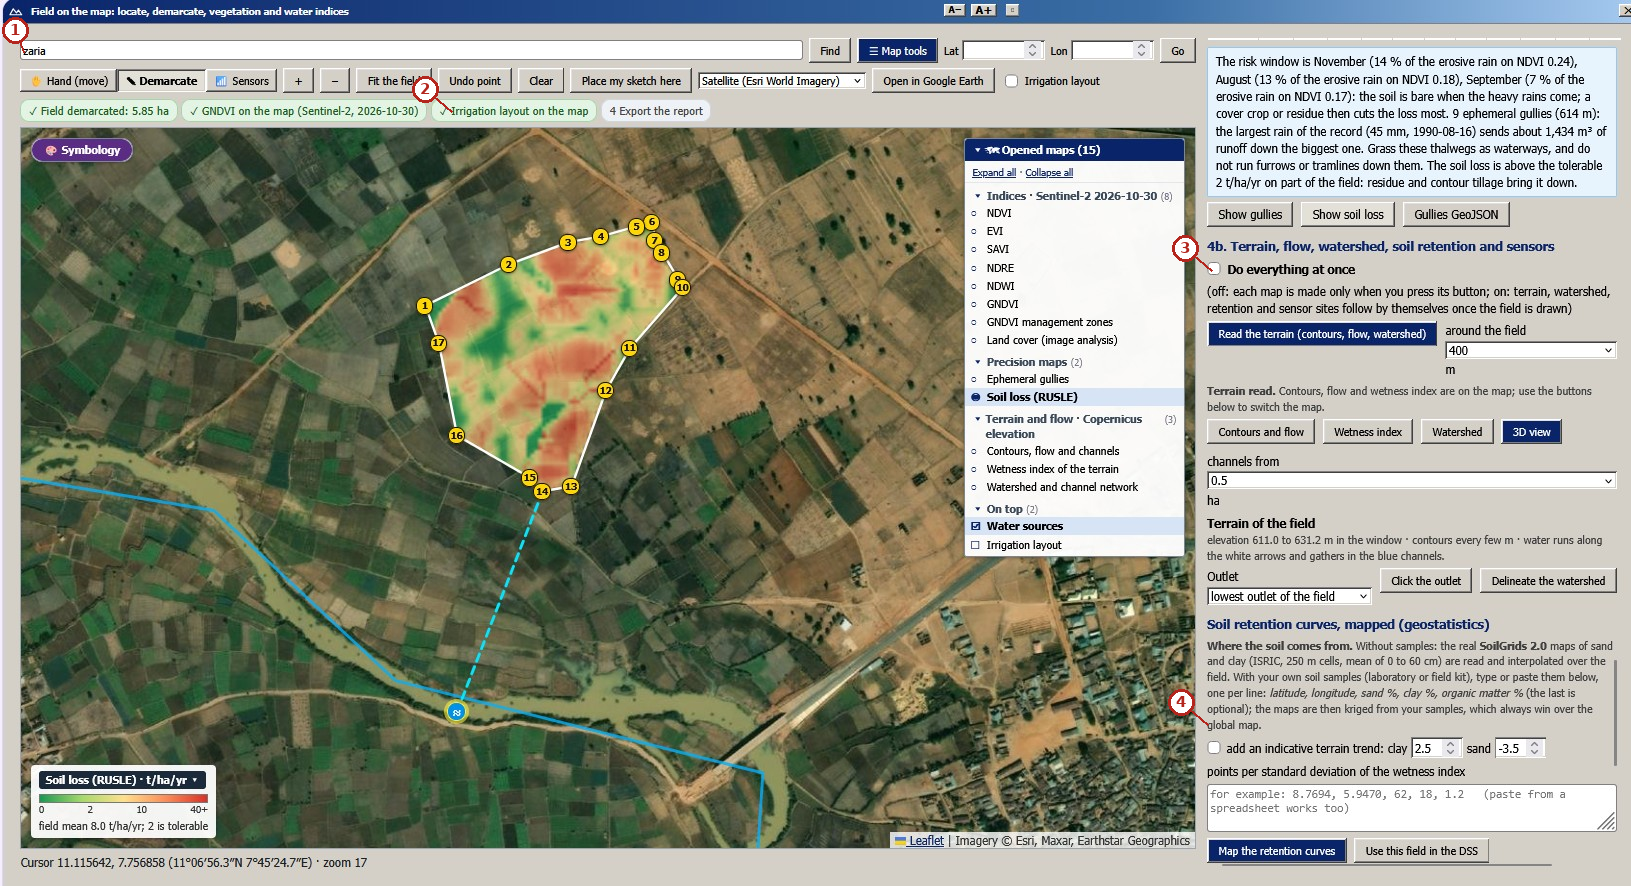
\includegraphics[width=\textwidth,height=0.42\textheight,keepaspectratio]{../figures/annot/p3_fig-zaria2_2.png}\end{center}

\textbf{What the numbered labels point to (picture 3 of 4: Soil loss (RUSLE), field mean 8.0~t\,ha$^{-1}$\,yr$^{-1}$, and the months of risk.).}
\begin{enumerate}[nosep,label=\protect\circled{\arabic*}]
\item ``Zaria'': a heading or control of this screen; the caption above says which layer it belongs to.
\item ``Irrigation layout on the map'': a heading or control of this screen; the caption above says which layer it belongs to.
\item ``Do everything at once'': a heading or control of this screen; the caption above says which layer it belongs to.
\item ``global map'': a heading or control of this screen; the caption above says which layer it belongs to.
\end{enumerate}

\begin{center}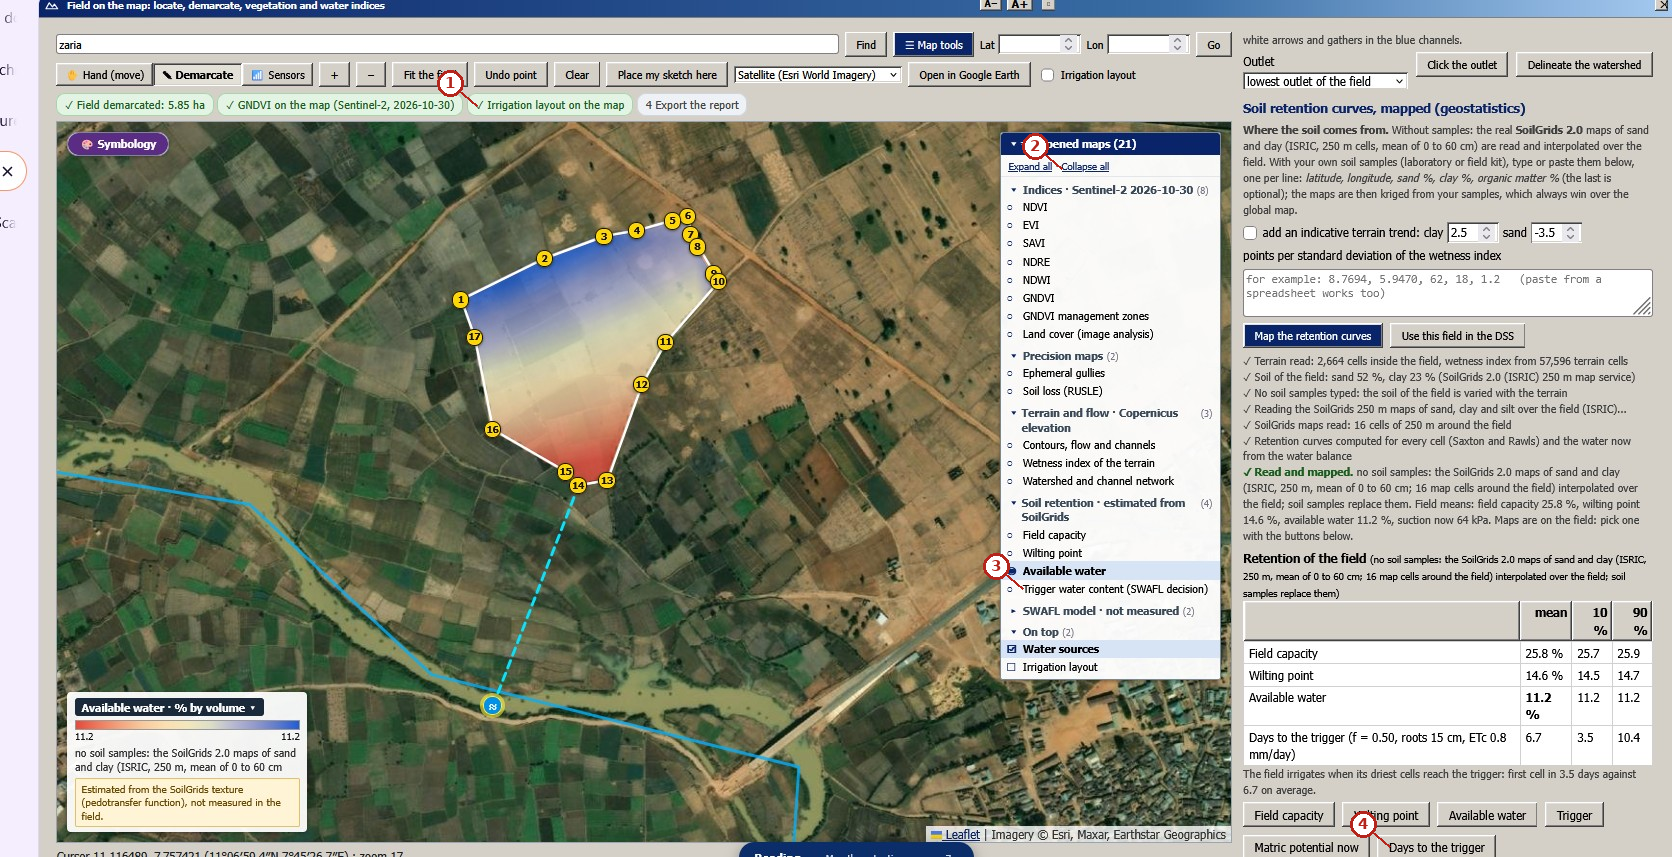
\includegraphics[width=\textwidth,height=0.42\textheight,keepaspectratio]{../figures/annot/p3_fig-zaria2_3.png}\end{center}

\textbf{What the numbered labels point to (picture 4 of 4: Available water from the retention curves mapped from SoilGrids (11.2\,\% by volume) and the days to the trigger.).}
\begin{enumerate}[nosep,label=\protect\circled{\arabic*}]
\item ``layout on the map'': a heading or control of this screen; the caption above says which layer it belongs to.
\item ``Collapse all'': a heading or control of this screen; the caption above says which layer it belongs to.
\item ``Trigger water content (SWAFL decision)'': a heading or control of this screen; the caption above says which layer it belongs to.
\item ``Days to the trigger'': the suction (or depletion) at which irrigation starts.
\end{enumerate}

\textbf{What it shows.} The same field: terrain, water source, erosion and soil water retention from open data (screen captures of release 1.1.0). Panels: (a) Contours every metre, flow arrows and channels, and the ranked water sources. (b) GNDVI and the line to the best water source, the Galma River (288~m). (c) Soil loss (RUSLE), field mean 8.0~t\,ha$^{-1}$\,yr$^{-1}$, and the months of risk. (d) Available water from the retention curves mapped from SoilGrids (11.2\,\% by volume) and the days to the trigger.

\textbf{How to read the labels, symbols and colours.} Screens: contours and flow, the best water source, soil loss and available water.

\textbf{What affects it, and why it happens.} Water flows down the steepest slope to the channels; soil loss is largest on steep, bare and erodible cells; available water follows soil texture. Water flows down the contours to channels; soil loss is highest on bare, steep, erosive cells; available water follows the texture mapped from SoilGrids.

\textbf{How it is made.} Screen capture of SWAFL Desktop 1.1.0 (not regenerated).


\subsection{Reading Figure 4 of the article}
\begin{center}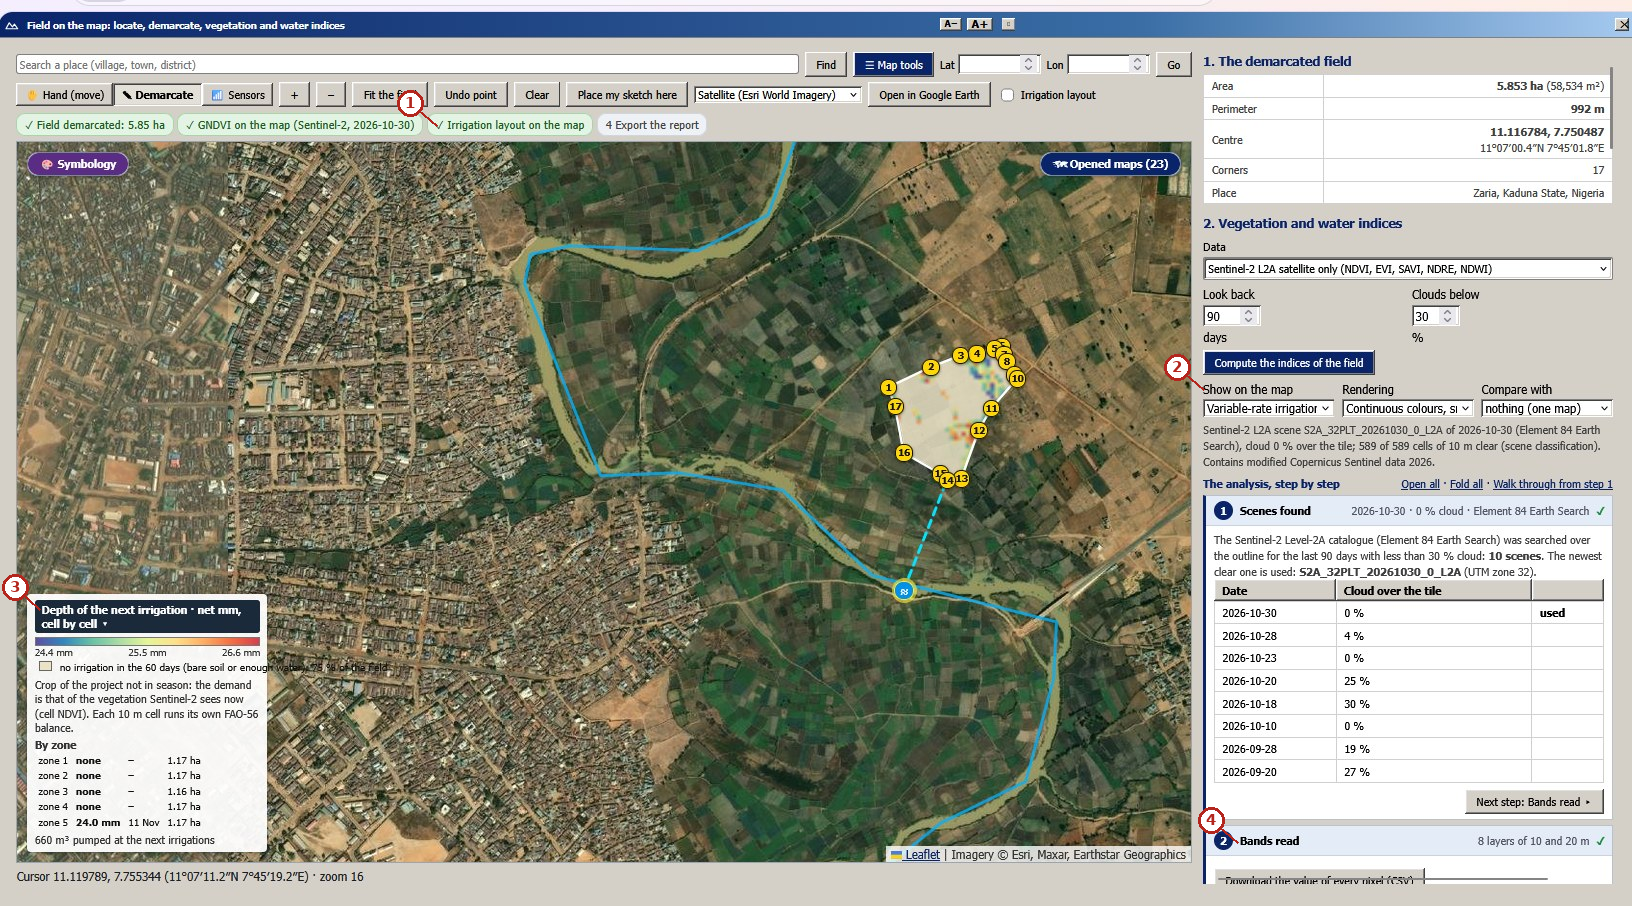
\includegraphics[width=\textwidth,height=0.42\textheight,keepaspectratio]{../figures/annot/p3_fig-zaria3_0.png}\end{center}

\textbf{What the numbered labels point to.}
\begin{enumerate}[nosep,label=\protect\circled{\arabic*}]
\item ``Irrigation layout on the map'': a heading or control of this screen; the caption above says which layer it belongs to.
\item ``Show on the map'': a heading or control of this screen; the caption above says which layer it belongs to.
\item ``Depth of the next'': a heading or control of this screen; the caption above says which layer it belongs to.
\item ``Bands read'': satellite indices of the vegetation computed from the Sentinel-2 bands.
\end{enumerate}

\textbf{What it shows.} Depth of the next irrigation on the Zaria field, cell by cell, from the FAO-56 balance of each 10\,m cell (real screenshot).

\textbf{How to read the labels, symbols and colours.} Map of the depth of the next irrigation, cell by cell, with a colour scale in mm.

\textbf{What affects it, and why it happens.} Cells with more green cover use more water and need deeper irrigation sooner. Cells with more vegetation (higher demand) or less available water need deeper irrigation sooner.

\textbf{How it is made.} Screen capture of SWAFL Desktop 1.1.0 (not regenerated).


\subsection{Reading Figure 5 of the article}
\begin{center}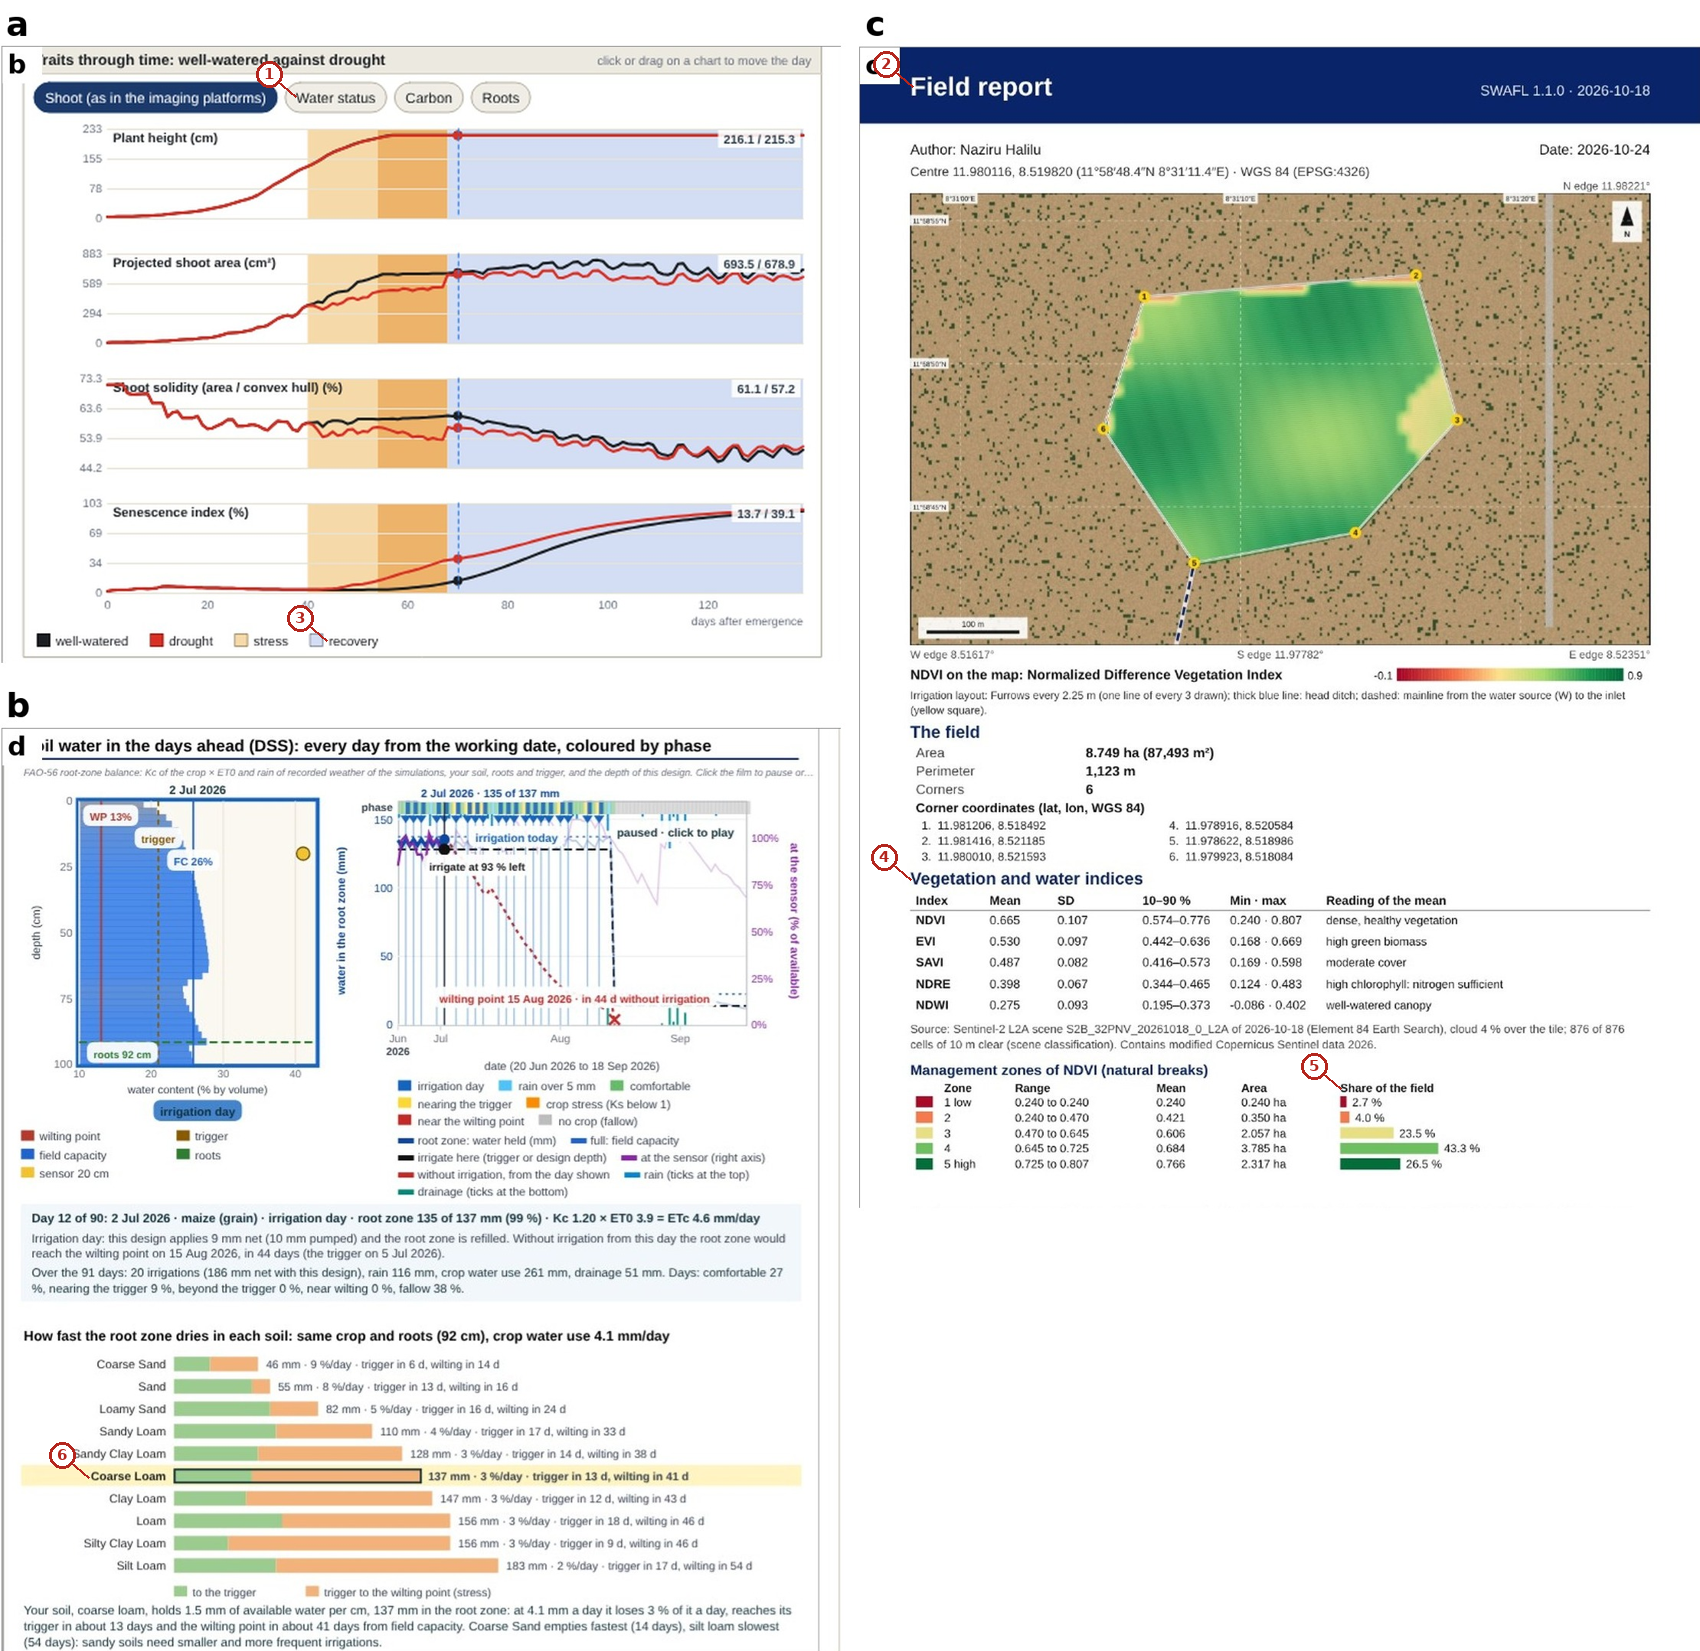
\includegraphics[width=\textwidth,height=0.42\textheight,keepaspectratio]{../figures/annot/p3_fig-pheno-screens_0.png}\end{center}

\textbf{What the numbered labels point to.}
\begin{enumerate}[nosep,label=\protect\circled{\arabic*}]
\item ``Water status Carbon Roots'': the roots: depth, density and uptake.
\item ``Field report'': export of the field report and its maps.
\item ``recovery'': a heading or control of this screen; the caption above says which layer it belongs to.
\item ``Vegetation and water indices'': satellite indices of the vegetation computed from the Sentinel-2 bands.
\item ``Share of the field'': a heading or control of this screen; the caption above says which layer it belongs to.
\item ``Coarse Loam'': the soil of the project, which every layer uses.
\end{enumerate}

\textbf{What it shows.} (a) Traits through time, well-watered against drought, with the phases of the stress marked. (b) Soil water in the days ahead with the irrigation decision of the design. (c) The field report (page 1).

\textbf{How to read the labels, symbols and colours.} (a) Traits through time, well-watered against drought; (b) soil water ahead with the decision; (c) the field report.

\textbf{What affects it, and why it happens.} Under drought the plant takes less water, closes stomata and grows less, so traits fall behind the well-watered plant. Traits fall behind under drought because uptake and growth fall with soil water.

\textbf{How it is made.} Screen capture of SWAFL Desktop 1.1.0 (not regenerated).


\subsection{Reading Figure 6 of the article}
\begin{center}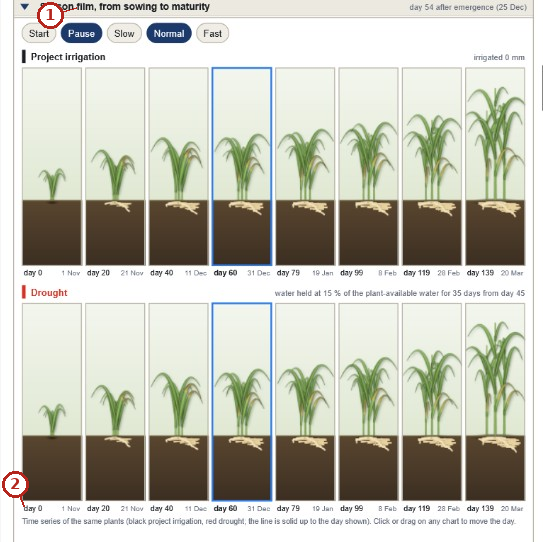
\includegraphics[width=\textwidth,height=0.42\textheight,keepaspectratio]{../figures/annot/p3_fig-season-film_0.png}\end{center}

\textbf{What the numbered labels point to.}
\begin{enumerate}[nosep,label=\protect\circled{\arabic*}]
\item ``film, from sowing to maturity'': a heading or control of this screen; the caption above says which layer it belongs to.
\item ``day 0'': a heading or control of this screen; the caption above says which layer it belongs to.
\end{enumerate}

\textbf{What it shows.} The season film of the phenotyping layer: the same plants from sowing to maturity every 20 days, under the irrigation of the project (top) and under a drought that holds the water at 15\,\% of the plant-available water for 35 days from day 45 (bottom), with shoots and roots drawn from the state of the model (screen capture of release 1.1.0).

\textbf{How to read the labels, symbols and colours.} The same plants every 20 days under the project's irrigation (top) and a drought (bottom).

\textbf{What affects it, and why it happens.} Water stress reduces growth and sends roots deeper, so the drought plants are smaller with deeper roots. Under drought the plants grow less and roots go deeper, as the model's water stress reduces growth.

\textbf{How it is made.} Screen capture of SWAFL Desktop 1.1.0 (not regenerated).


\subsection{Reading Figure 7 of the article}
\begin{center}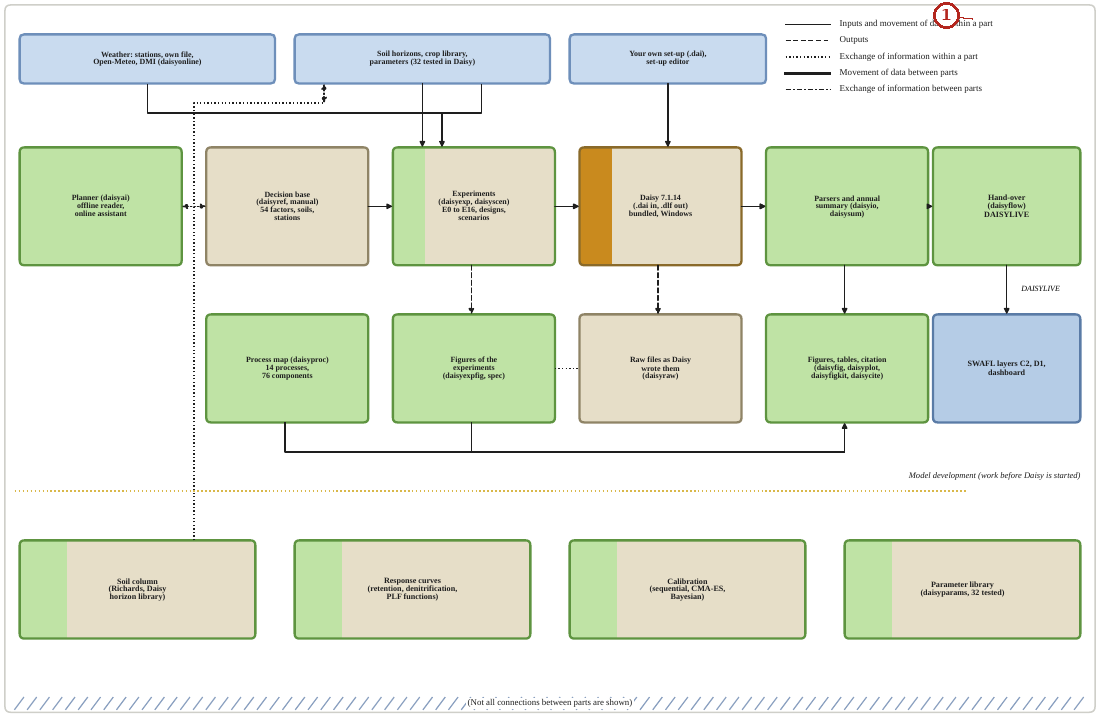
\includegraphics[width=\textwidth,height=0.42\textheight,keepaspectratio]{../figures/annot/p3_fig-wb_0.png}\end{center}

\textbf{What the numbered labels point to.}
\begin{enumerate}[nosep,label=\protect\circled{\arabic*}]
\item Panel (a): see the caption above.
\end{enumerate}

\textbf{What it shows.} Modules of the Daisy workbench and the hand-over. The chain runs from the planner and the decision base through the experiments, Daisy and the parsers to the hand-over; the modules below the dotted line are used before Daisy is started.

\textbf{How to read the labels, symbols and colours.} Modules of the workbench and the hand-over; the dotted line separates what runs before Daisy.

\textbf{What affects it, and why it happens.} A question becomes a checked design, Daisy runs, the logs are parsed and handed to the layers.

\textbf{How it is made.} Figure drawn by the script from the input data. Script: \nolinkurl{Manuscripts/reproducibility/p456/p456_figs_architecture.py}. Input: \nolinkurl{Data/daisy_ensemble.csv.gz}.


\subsection{Reading Figure 10 of the article}
\begin{center}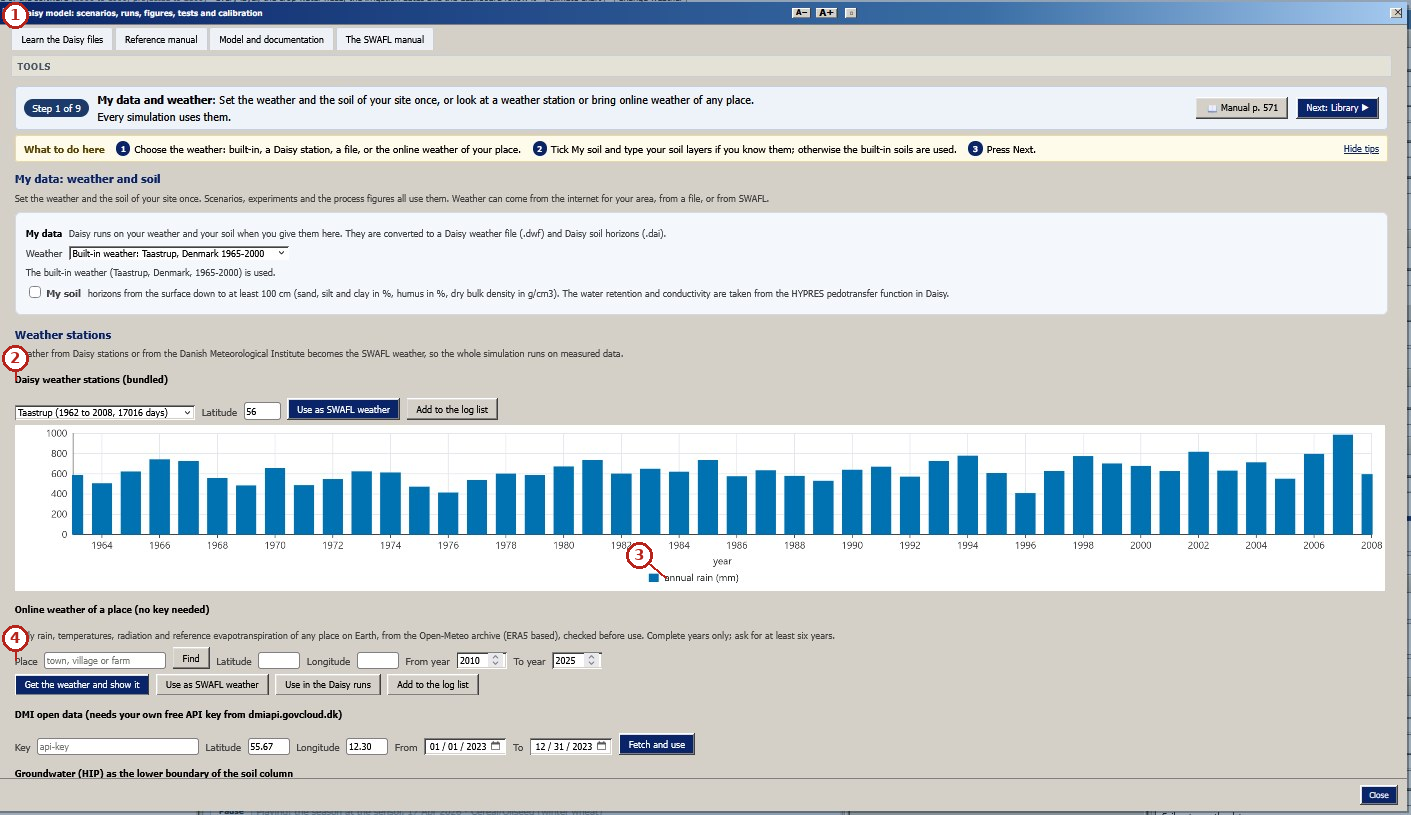
\includegraphics[width=\textwidth,height=0.42\textheight,keepaspectratio]{../figures/annot/p3_fig-wbsteps_0.png}\end{center}

\textbf{What the numbered labels point to (picture 1 of 8: Step 1: my data and weather (manual p.~760).).}
\begin{enumerate}[nosep,label=\protect\circled{\arabic*}]
\item ``Daisy runs, figures, tests and calibration'': the Daisy model and its workbench.
\item ``Daisy weather stations (bundled)'': the Daisy model and its workbench.
\item ``annual rain (mm)'': rain, from the weather of the project.
\item ``Place'': a heading or control of this screen; the caption above says which layer it belongs to.
\end{enumerate}

\begin{center}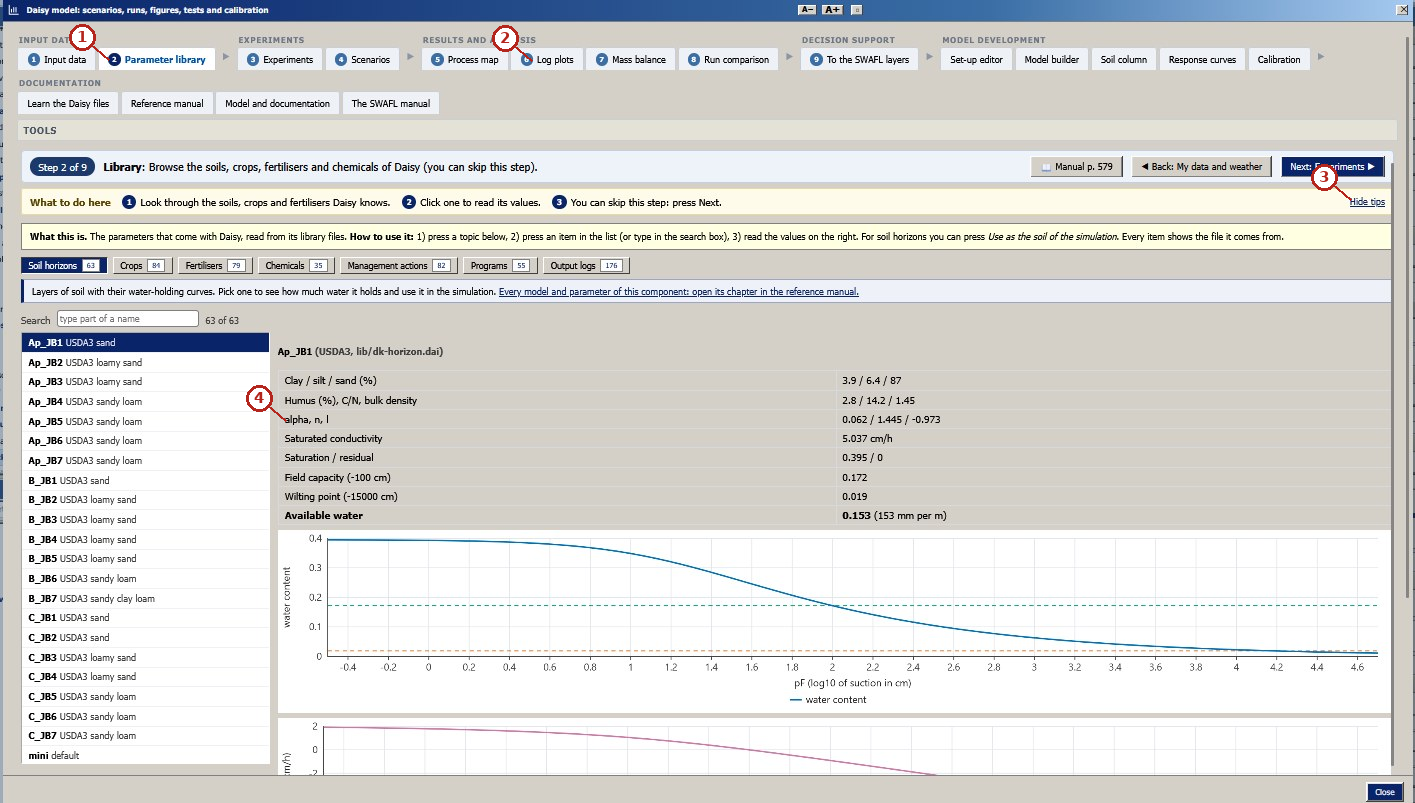
\includegraphics[width=\textwidth,height=0.42\textheight,keepaspectratio]{../figures/annot/p3_fig-wbsteps_1.png}\end{center}

\textbf{What the numbered labels point to (picture 2 of 8: Step 2: library of soils, crops and fertilisers (p.~583).).}
\begin{enumerate}[nosep,label=\protect\circled{\arabic*}]
\item ``Parameter library'': a heading or control of this screen; the caption above says which layer it belongs to.
\item ``Leg plots'': a heading or control of this screen; the caption above says which layer it belongs to.
\item ``Hide tos'': a heading or control of this screen; the caption above says which layer it belongs to.
\item ``alpha, n'': a heading or control of this screen; the caption above says which layer it belongs to.
\end{enumerate}

\begin{center}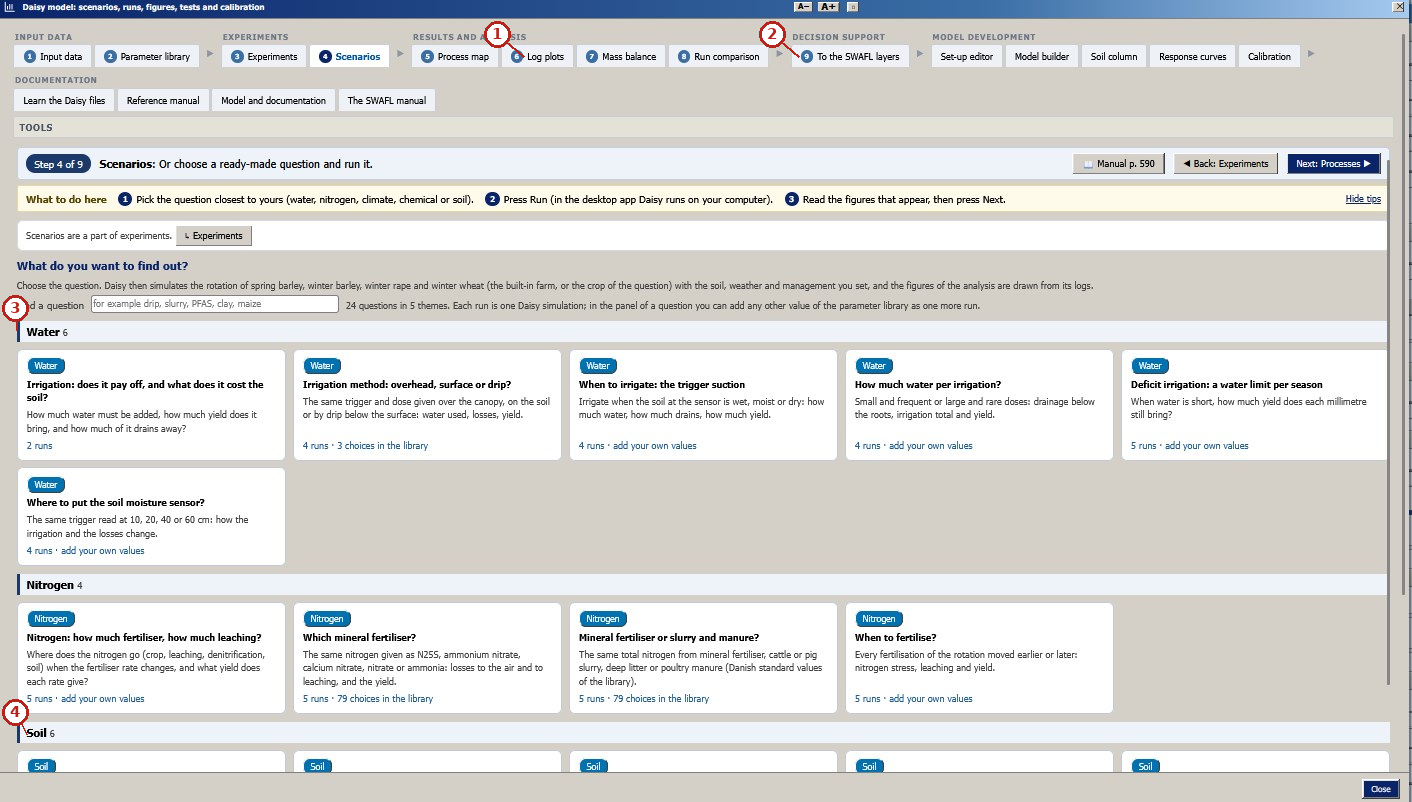
\includegraphics[width=\textwidth,height=0.42\textheight,keepaspectratio]{../figures/annot/p3_fig-wbsteps_2.png}\end{center}

\textbf{What the numbered labels point to (picture 3 of 8: Step 4: scenarios, a question and its runs (p.~762).).}
\begin{enumerate}[nosep,label=\protect\circled{\arabic*}]
\item ``Log plots'': a heading or control of this screen; the caption above says which layer it belongs to.
\item ``SWAFL layers'': the menu bar of the program (file, view, run, Daisy, help).
\item ``water'': a heading or control of this screen; the caption above says which layer it belongs to.
\item ``Soil 6'': the soil of the project, which every layer uses.
\end{enumerate}

\begin{center}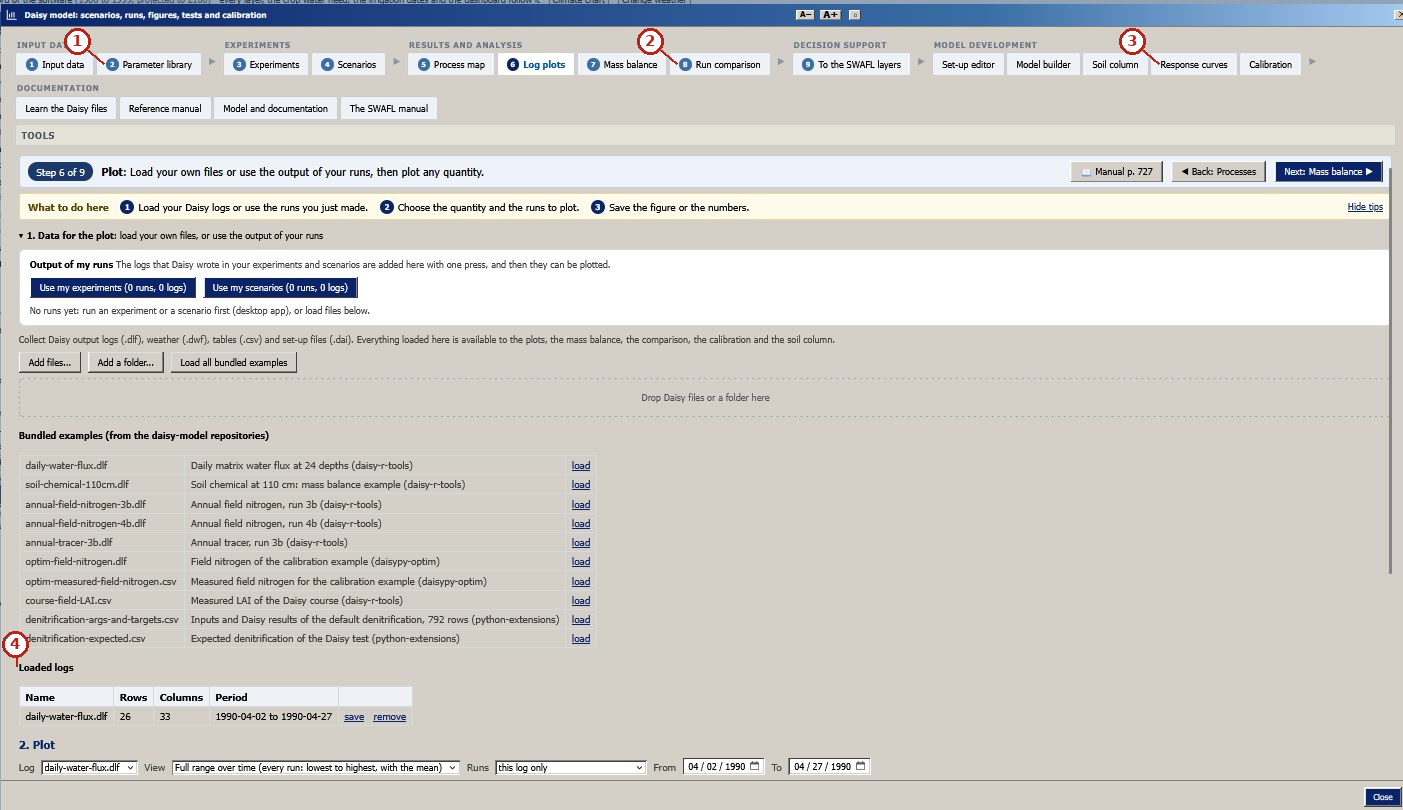
\includegraphics[width=\textwidth,height=0.42\textheight,keepaspectratio]{../figures/annot/p3_fig-wbsteps_3.png}\end{center}

\textbf{What the numbered labels point to (picture 4 of 8: Step 6: log plots of the runs (p.~763).).}
\begin{enumerate}[nosep,label=\protect\circled{\arabic*}]
\item ``Parameter library'': a heading or control of this screen; the caption above says which layer it belongs to.
\item ``Run comparison'': a heading or control of this screen; the caption above says which layer it belongs to.
\item ``Response curves'': a heading or control of this screen; the caption above says which layer it belongs to.
\item ``Loaded logs'': a heading or control of this screen; the caption above says which layer it belongs to.
\end{enumerate}

\begin{center}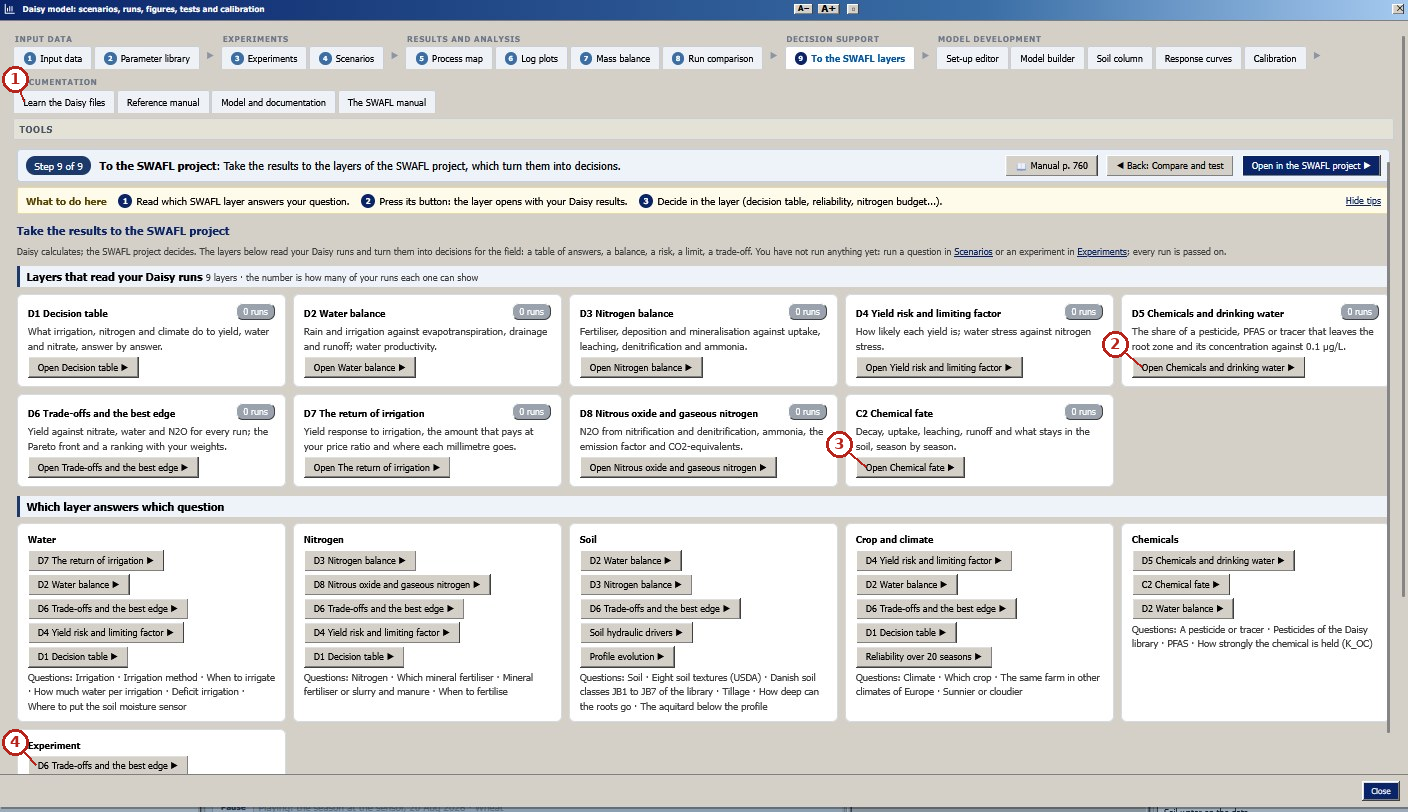
\includegraphics[width=\textwidth,height=0.42\textheight,keepaspectratio]{../figures/annot/p3_fig-wbsteps_4.png}\end{center}

\textbf{What the numbered labels point to (picture 5 of 8: Step 9: to the SWAFL layers, which layer answers which question (p.~764).).}
\begin{enumerate}[nosep,label=\protect\circled{\arabic*}]
\item ``Learn the Daisy files'': the Daisy model and its workbench.
\item ``Open Chemicals and drinking'': a heading or control of this screen; the caption above says which layer it belongs to.
\item ``Open Chemical'': a heading or control of this screen; the caption above says which layer it belongs to.
\item ``D6 and the best edge'': a heading or control of this screen; the caption above says which layer it belongs to.
\end{enumerate}

\begin{center}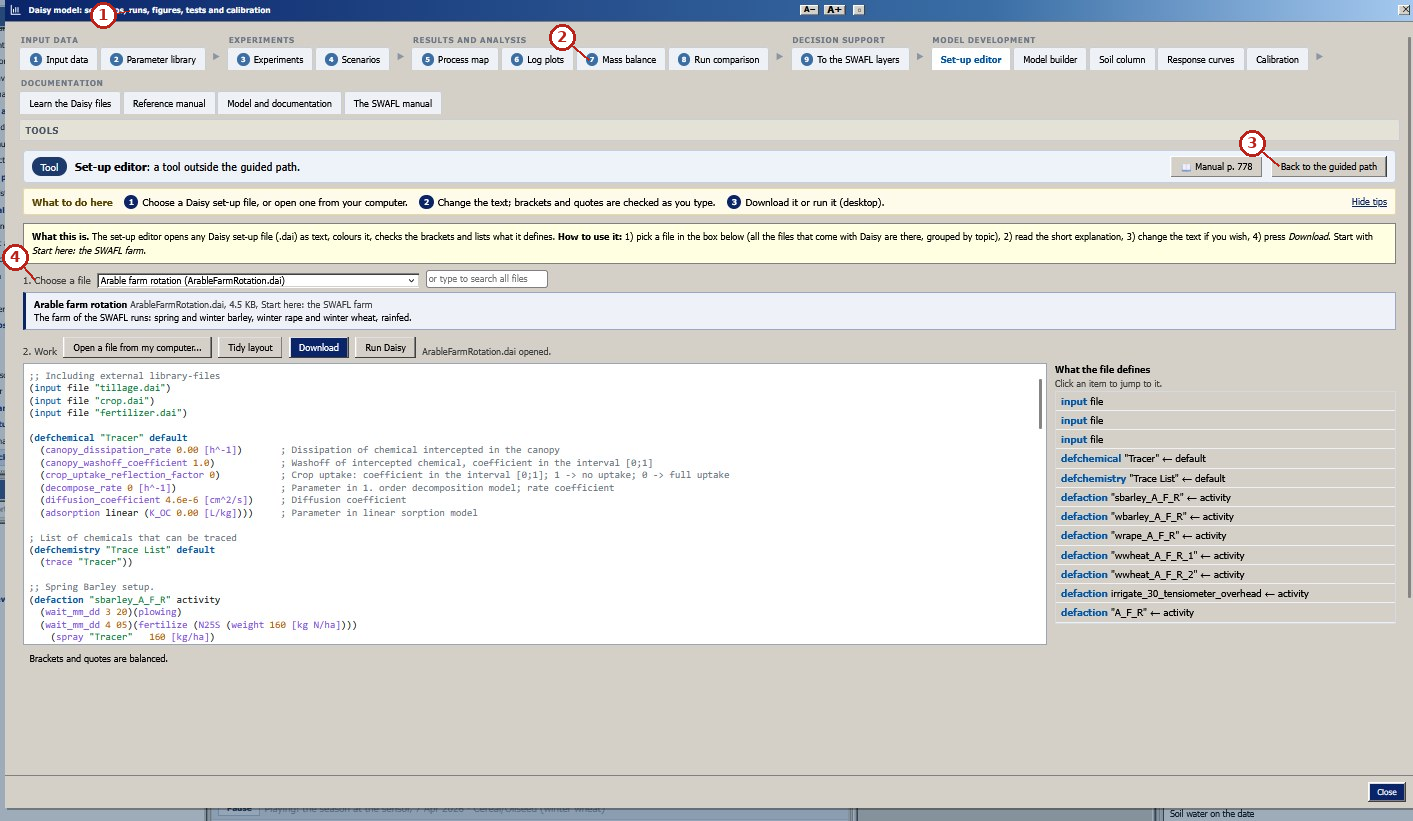
\includegraphics[width=\textwidth,height=0.42\textheight,keepaspectratio]{../figures/annot/p3_fig-wbsteps_5.png}\end{center}

\textbf{What the numbered labels point to (picture 6 of 8: Tool: set-up editor with bracket check (p.~783).).}
\begin{enumerate}[nosep,label=\protect\circled{\arabic*}]
\item ``runs, figures, tests and cal'': a heading or control of this screen; the caption above says which layer it belongs to.
\item ``Mass balance'': a heading or control of this screen; the caption above says which layer it belongs to.
\item ``Back to the guided path'': moves to the next or previous step of the guided path.
\item ``Choose file farm rotation'': a heading or control of this screen; the caption above says which layer it belongs to.
\end{enumerate}

\begin{center}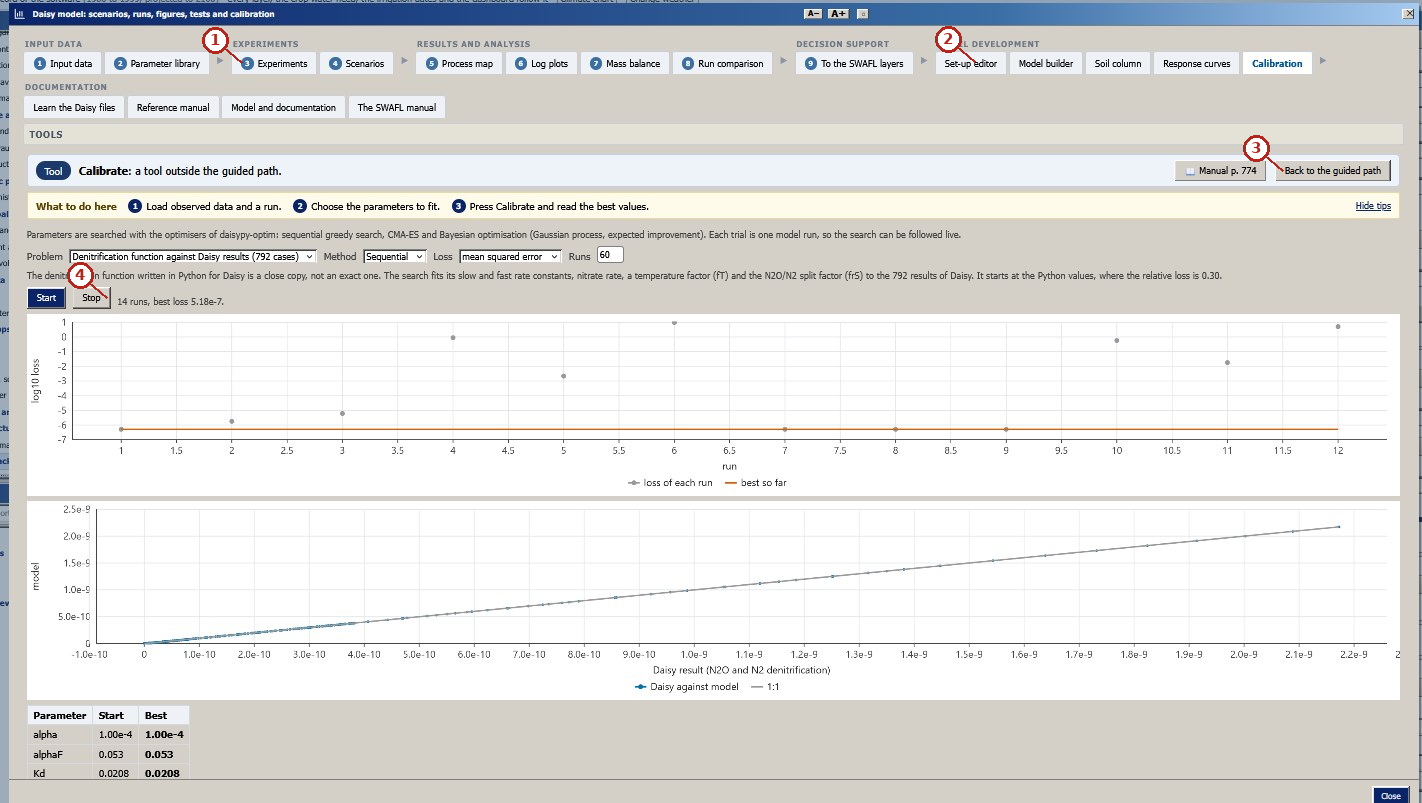
\includegraphics[width=\textwidth,height=0.42\textheight,keepaspectratio]{../figures/annot/p3_fig-wbsteps_6.png}\end{center}

\textbf{What the numbered labels point to (picture 7 of 8: Tool: calibration (daisypy-optim) (p.~779).).}
\begin{enumerate}[nosep,label=\protect\circled{\arabic*}]
\item ``Experiments Scenarios'': a heading or control of this screen; the caption above says which layer it belongs to.
\item ``editor builder'': a heading or control of this screen; the caption above says which layer it belongs to.
\item ``Back to the guided path'': moves to the next or previous step of the guided path.
\item ``14 runs, best loss'': a heading or control of this screen; the caption above says which layer it belongs to.
\end{enumerate}

\begin{center}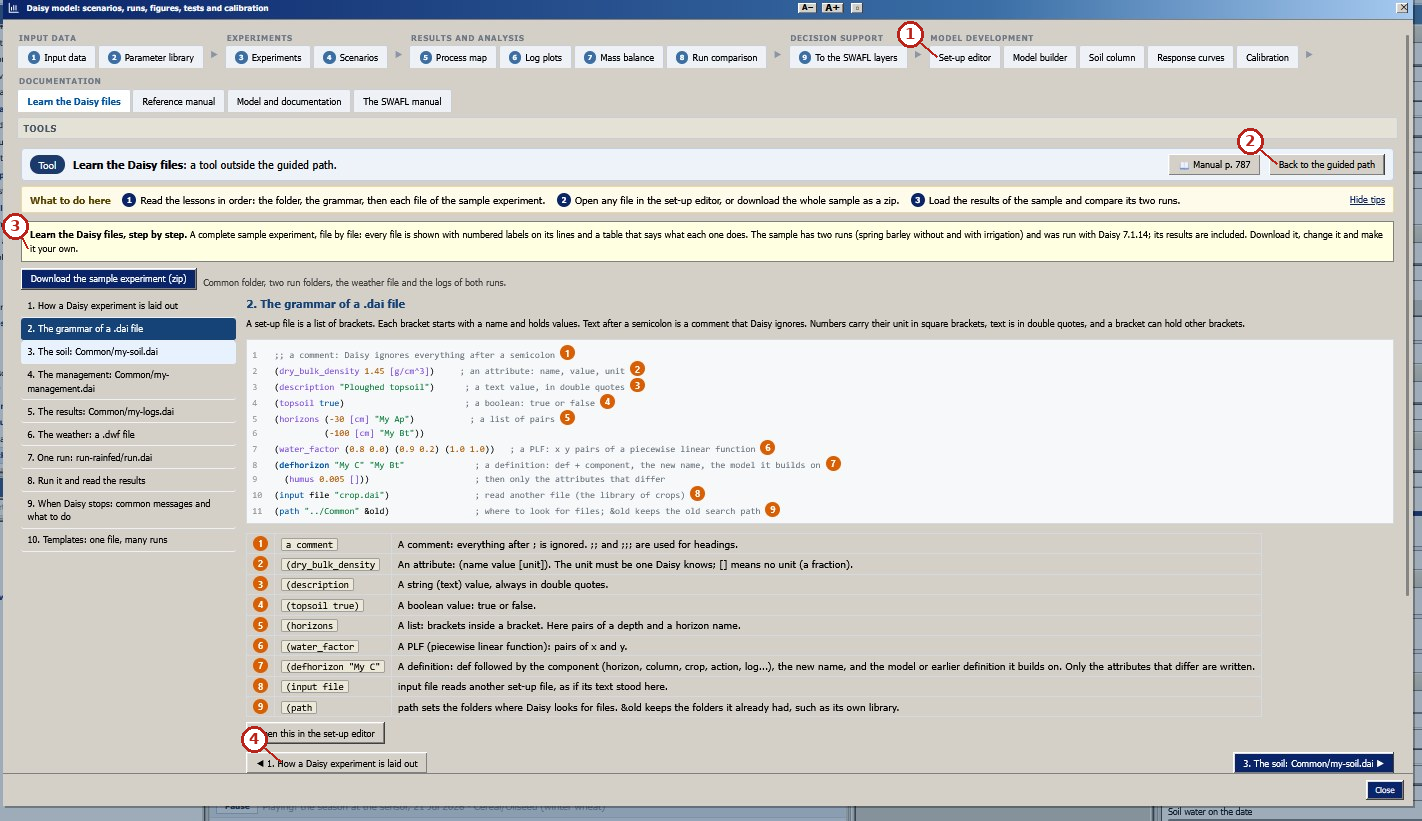
\includegraphics[width=\textwidth,height=0.42\textheight,keepaspectratio]{../figures/annot/p3_fig-wbsteps_7.png}\end{center}

\textbf{What the numbered labels point to (picture 8 of 8: Tool: learn the Daisy files, the grammar of a .dai file (p.~792).).}
\begin{enumerate}[nosep,label=\protect\circled{\arabic*}]
\item ``Setup editor'': a heading or control of this screen; the caption above says which layer it belongs to.
\item ``Back to the guided path'': moves to the next or previous step of the guided path.
\item ``it your own'': a heading or control of this screen; the caption above says which layer it belongs to.
\item ``How a Daisy out'': the Daisy model and its workbench.
\end{enumerate}

\textbf{What it shows.} The guided path of the Daisy workbench and three of its tools (real screenshots of release 1.1.0). Each step carries its step number, a one-line ``what to do here'', the manual page and Back and Next buttons. Panels: (a) Step 1: my data and weather (manual p.~760). (b) Step 2: library of soils, crops and fertilisers (p.~583). (c) Step 4: scenarios, a question and its runs (p.~762). (d) Step 6: log plots of the runs (p.~763). (e) Step 9: to the SWAFL layers, which layer answers which question (p.~764). (f) Tool: set-up editor with bracket check (p.~783). (g) Tool: calibration (daisypy-optim) (p.~779). (h) Tool: learn the Daisy files, the grammar of a .dai file (p.~792).

\textbf{How to read the labels, symbols and colours.} Eight screens of the guided path and tools, each with its manual page.

\textbf{What affects it, and why it happens.} The guided path orders the work from data to decision; each step opens the manual page that documents it. The path leads a user from data to decision in nine steps.

\textbf{How it is made.} Screen capture of SWAFL Desktop 1.1.0 (not regenerated).


\subsection{Reading Figure 11 of the article}
\begin{center}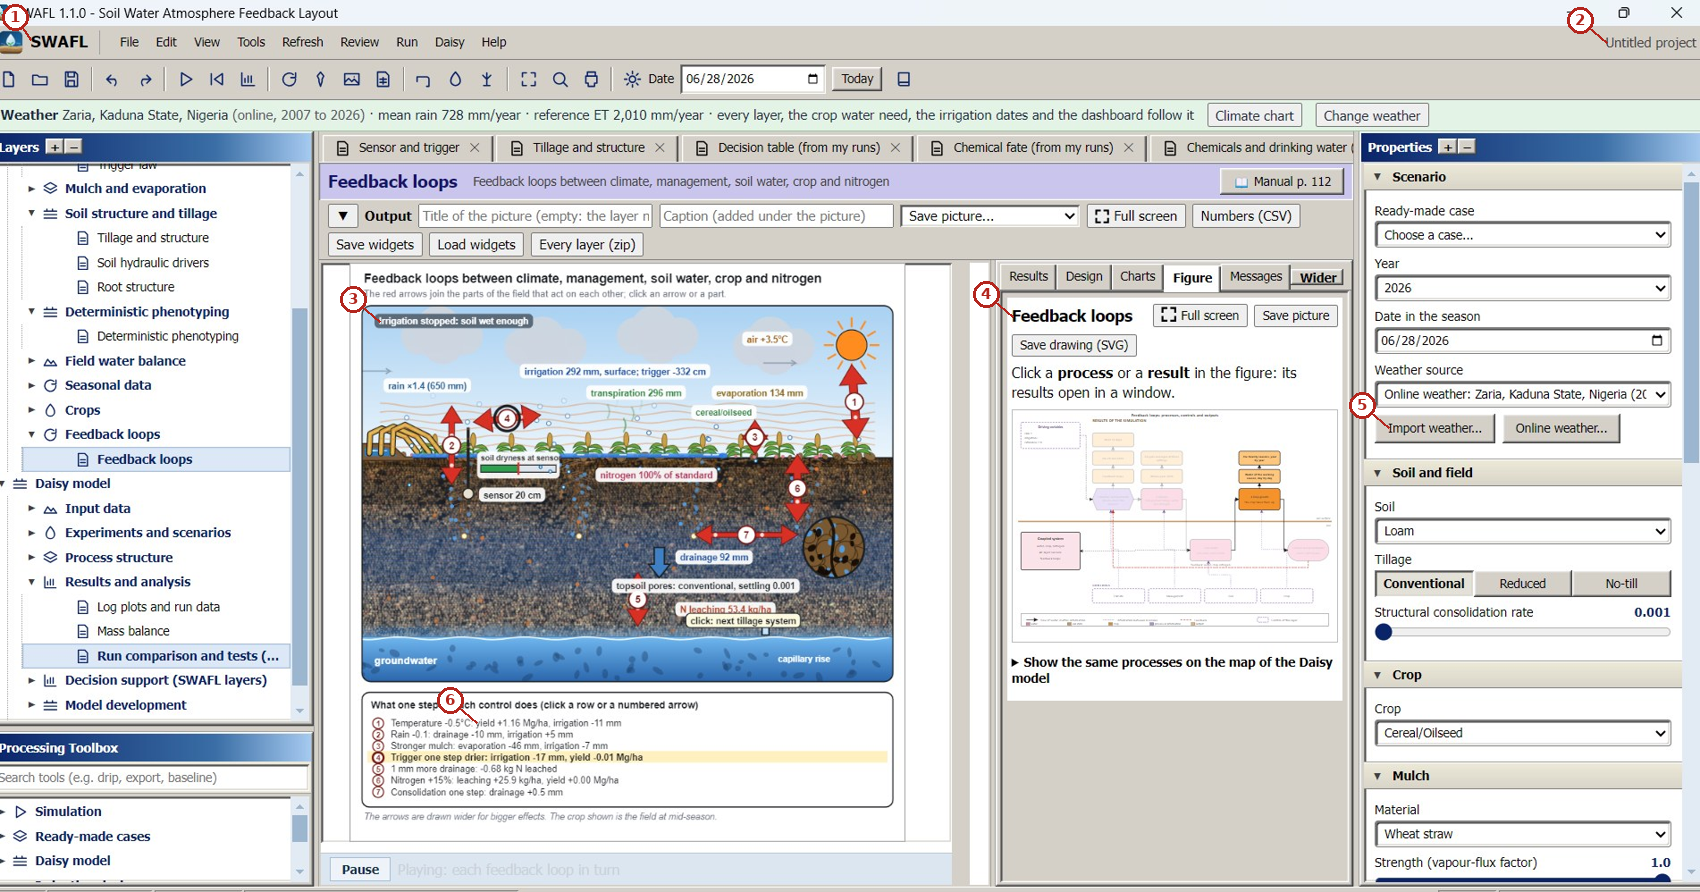
\includegraphics[width=\textwidth,height=0.42\textheight,keepaspectratio]{../figures/annot/p3_fig-mainzaria_0.png}\end{center}

\textbf{What the numbered labels point to.}
\begin{enumerate}[nosep,label=\protect\circled{\arabic*}]
\item ``SWAFL Tools Run Daisy Help'': the menu bar of the program (file, view, run, Daisy, help).
\item ``Untitled project'': a heading or control of this screen; the caption above says which layer it belongs to.
\item ``Irrigation stopped: soil wet enough'': the soil of the project, which every layer uses.
\item ``Feedback loops Full screen'': the feedback loops between climate, management, soil water, crop and nitrogen.
\item ``Import weather... Online weather'': the weather of the project: built-in record, a file of the user or online weather of any place.
\item ``yield irrigation -11 mm'': a heading or control of this screen; the caption above says which layer it belongs to.
\end{enumerate}

\textbf{What it shows.} The main window with the online weather of Zaria, Nigeria (2007--2026): Layers tree, the feedback-loops layer with the controls of the season, the Properties panel and the Processing toolbox (real screenshot).

\textbf{How to read the labels, symbols and colours.} Main window: Layers tree, feedback layer, Properties panel, toolbox.

\textbf{What affects it, and why it happens.} The Properties panel sets the soil, crop, mulch and weather that every layer uses, so changing it redraws the layer. Controls in the Properties panel drive every layer at once.

\textbf{How it is made.} Screen capture of SWAFL Desktop 1.1.0 (not regenerated).


\subsection{Reading Figure 21 of the article}
\begin{center}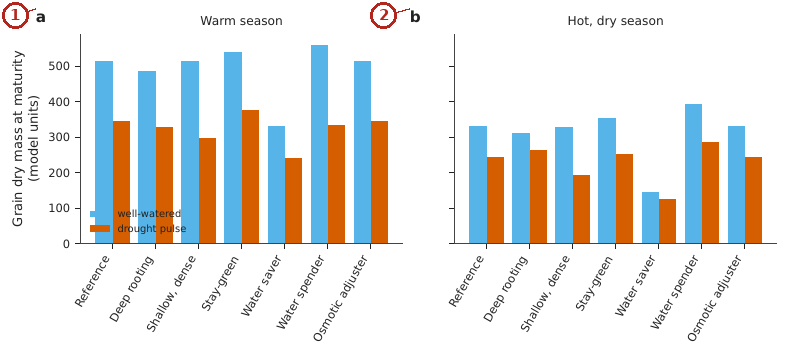
\includegraphics[width=\textwidth,height=0.42\textheight,keepaspectratio]{../figures/annot/p3_fig-pheno_0.png}\end{center}

\textbf{What the numbered labels point to.}
\begin{enumerate}[nosep,label=\protect\circled{\arabic*}]
\item Panel (a): and a hot, dry. \emph{Why:} Drought shortens grain filling, so grain mass falls; genotypes differ in how much.
\item Panel (b): season. \emph{Why:} Heat and dryness add to the drought effect, so all genotypes lose more.
\end{enumerate}

\textbf{What it shows.} Grain dry mass at maturity of seven genotypes, well-watered and under a drought pulse, in a warm (a) and a hot, dry (b) season.

\textbf{How to read the labels, symbols and colours.} Grain mass of seven genotypes, well-watered against drought, in a warm (a) and a hot, dry (b) season.

\textbf{What affects it, and why it happens.} Drought and heat shorten the grain-filling period and reduce assimilation, so all genotypes lose grain, by different amounts.

\textbf{How it is made.} Figure drawn by the script from the input data. Script: \nolinkurl{Manuscripts/reproducibility/p456/p456_figs_data.py}. Input: \nolinkurl{Data/daisy_ensemble.csv.gz}.


\subsection{Reading Figure 22 of the article}
\begin{center}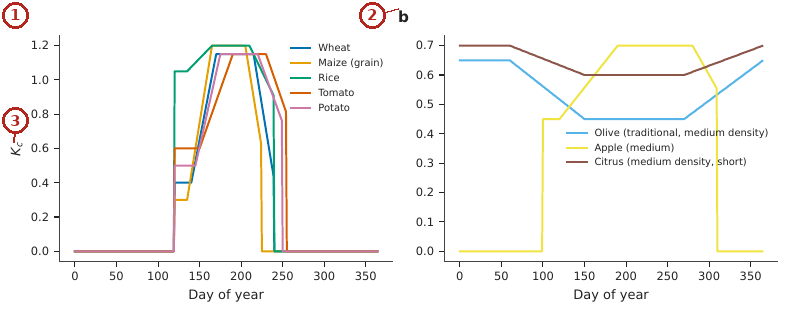
\includegraphics[width=\textwidth,height=0.42\textheight,keepaspectratio]{../figures/annot/p3_fig-crops_0.png}\end{center}

\textbf{What the numbered labels point to.}
\begin{enumerate}[nosep,label=\protect\circled{\arabic*}]
\item Panel (a): five annual crops. \emph{Why:} Coefficients rise with canopy cover, stay at the mid-season value and fall with senescence.
\item Panel (b): three perennial crops (medium density). \emph{Why:} Perennial crops keep a canopy most of the year, so the curves stay high longer.
\item Panel (c): see the caption above.
\end{enumerate}

\textbf{What it shows.} Daily crop coefficient curves of the library (Eq.~(2) of the article) at the default sowing date, (a) five annual crops, (b) three perennial crops (medium density).

\textbf{How to read the labels, symbols and colours.} Daily crop coefficient curves of the library crops at the default sowing date.

\textbf{What affects it, and why it happens.} Coefficients rise with canopy development to a mid-season plateau and fall with senescence (FAO-56).

\textbf{How it is made.} Figure drawn by the script from the input data. Script: \nolinkurl{Manuscripts/reproducibility/p456/p456_figs_data.py}. Input: \nolinkurl{Data/daisy_ensemble.csv.gz}.

\subsection{Derivation: Normalised spectral indices}\label{der:s3:1}
Green leaves absorb red light for photosynthesis and scatter near-infrared light in the leaf mesophyll. The normalised difference $\mathrm{NDVI}=(\rho_N-\rho_R)/(\rho_N+\rho_R)$ is a contrast of the two that is bounded in $[-1,1]$ and cancels a common multiplicative illumination factor $k$: $(k\rho_N-k\rho_R)/(k\rho_N+k\rho_R)$ equals NDVI. SAVI adds a soil term $L$ to the denominator to reduce the influence of bright soil, $(1+L)(\rho_N-\rho_R)/(\rho_N+\rho_R+L)$; EVI corrects for the atmosphere with the blue band and for the canopy background; the water indices use the shortwave-infrared band, which liquid water absorbs.


\subsection{Derivation: Crop coefficient through the season}\label{der:s3:2}
The FAO-56 curve is piecewise linear in time: constant $K_{ini}$ during the initial stage $L_1$, a linear rise to $K_{mid}$ over the development stage $L_2$, constant over the mid-season $L_3$ and a linear fall to $K_{end}$ over the late stage $L_4$ \citep{Allen1998}. The crop evapotranspiration is $\ET_c=K_c\,\ET_0$.


\subsection{Derivation: Daily root-zone balance of each map cell}\label{der:s3:3}
For each cell, the root-zone depletion follows $D_{r,i}=D_{r,i-1}-(P-\mathrm{RO})_i-I_i+\ET_{c,i}+\mathrm{DP}_i$, bounded by $0\le D_{r}\le\TAW$; deep percolation occurs only when the depletion would fall below zero. Irrigation is required when $D_r$ exceeds the readily available water $p\,\TAW$; the net depth to apply is $D_r$ \citep{Allen1998}.


\subsection{Derivation: Terrain, flow and wetness}\label{der:s3:7}
On a filled elevation grid each cell drains to the steepest of its eight neighbours (D8). The upslope area $A$ of a cell is the sum of the areas that drain through it, and the specific area is $a=A/w$ with $w$ the cell width. The topographic wetness index $\ln(a/\tan\beta)$ is large where much water arrives and the slope $\beta$ is small, which marks where the soil stays wet.


\subsection{Derivation: Soil loss}\label{der:s3:8}
The revised universal soil loss equation multiplies the rain erosivity $R$, the soil erodibility $K$, the slope length and steepness $LS$, the cover $C$ and the practice $P$: $A=R\,K\,LS\,C\,P$ in t\,ha$^{-1}$\,yr$^{-1}$ \citep{Renard1994}.


